% Biên dịch bằng XeLaTeX + Biber (Overleaf: Menu > Compiler = XeLaTeX).
\documentclass[12pt,a4paper]{report}

\usepackage{fontspec}
% TeX Gyre Termes (tương đương Times New Roman), nạp theo tên file để chạy được cả MiKTeX lẫn Overleaf
\setmainfont{texgyretermes}[Extension=.otf, UprightFont=*-regular, BoldFont=*-bold,
  ItalicFont=*-italic, BoldItalicFont=*-bolditalic]
\usepackage[vietnamese]{babel}
\usepackage[a4paper,left=3cm,right=2cm,top=2.5cm,bottom=2.5cm]{geometry}
\usepackage{amsmath,amssymb}
\usepackage{graphicx,booktabs,array,enumitem,setspace}
\usepackage[labelsep=period]{caption}
\usepackage{titlesec,tocloft}
\usepackage{tikz}  % viền trang bìa
\usetikzlibrary{calc}
\usepackage[backend=biber,style=ieee,sorting=none,language=american]{biblatex}
\addbibresource{references.bib}
% Cho phép ngắt URL dài trong tài liệu tham khảo ở chữ thường, chữ hoa và chữ số
\setcounter{biburllcpenalty}{7000}
\setcounter{biburlucpenalty}{8000}
\setcounter{biburlnumpenalty}{9000}
\DeclareLanguageMapping{vietnamese}{english}
\usepackage[colorlinks=true,linkcolor=black,citecolor=blue,urlcolor=blue]{hyperref}

\onehalfspacing
\setlength{\parindent}{1cm}
\setlength{\parskip}{0pt}
\numberwithin{equation}{chapter}
\setcounter{secnumdepth}{3}
\setcounter{tocdepth}{2}
\setlist{nosep,leftmargin=1.5cm}

% Tiêu đề chương / mục
\titleformat{\chapter}[block]{\centering\bfseries\large}{CHƯƠNG \thechapter.}{0.4em}{}
\titleformat{name=\chapter,numberless}[block]{\centering\bfseries\large}{}{0pt}{}
\titlespacing*{\chapter}{0pt}{0pt}{18pt}
\titleformat{\section}{\bfseries\large}{\thesection.}{0.5em}{}
\titleformat{name=\section,numberless}{\bfseries\large}{}{0pt}{}
\titleformat{\subsection}{\bfseries\normalsize}{\thesubsection.}{0.5em}{}

% Mục lục
\addto\captionsvietnamese{%  babel ghi đè nếu đặt trực tiếp
  \renewcommand{\contentsname}{MỤC LỤC}%
  \renewcommand{\listfigurename}{DANH MỤC HÌNH}%
  \renewcommand{\listtablename}{DANH MỤC BẢNG}}
\renewcommand{\cftchappresnum}{CHƯƠNG }
\renewcommand{\cftchapaftersnum}{.}
% Tiêu đề mục lục, danh mục hình, danh mục bảng căn giữa như tiêu đề chương
\renewcommand{\cfttoctitlefont}{\hspace*{\fill}\bfseries\large}
\renewcommand{\cftaftertoctitle}{\hspace*{\fill}}
\renewcommand{\cftloftitlefont}{\hspace*{\fill}\bfseries\large}
\renewcommand{\cftafterloftitle}{\hspace*{\fill}}
\renewcommand{\cftlottitlefont}{\hspace*{\fill}\bfseries\large}
\renewcommand{\cftafterlottitle}{\hspace*{\fill}}
\setlength{\cftbeforetoctitleskip}{0pt}
\setlength{\cftbeforeloftitleskip}{0pt}
\setlength{\cftbeforelottitleskip}{0pt}
\renewcommand{\cftfigpresnum}{Hình }
\renewcommand{\cfttabpresnum}{Bảng }
\setlength{\cftfignumwidth}{5em}
\setlength{\cfttabnumwidth}{5.5em}
\setlength{\cftchapnumwidth}{6.5em}
\renewcommand{\cftchapfont}{\bfseries}
\renewcommand{\cftchapleader}{\bfseries\cftdotfill{\cftdotsep}}
\renewcommand{\cftchappagefont}{\bfseries}

\begin{document}

% Lề riêng cho bìa: đối xứng để chữ nằm giữa khung, đủ xa hoa văn ở các góc
\newgeometry{left=3cm,right=3cm,top=3.6cm,bottom=3.6cm}
\begin{titlepage}
% Viền hoa văn theo mẫu bìa của trường (ảnh lấy từ bìa báo cáo mẫu), giữ tỷ lệ, đặt giữa trang.
% vien_bia_xanh.png: như vien_bia.jpg nhưng khung ngoài tô màu xanhbien, hoa văn giữ màu đen
\definecolor{xanhbien}{RGB}{0,51,153}
\begin{tikzpicture}[remember picture, overlay]
  \node at (current page.center)
    {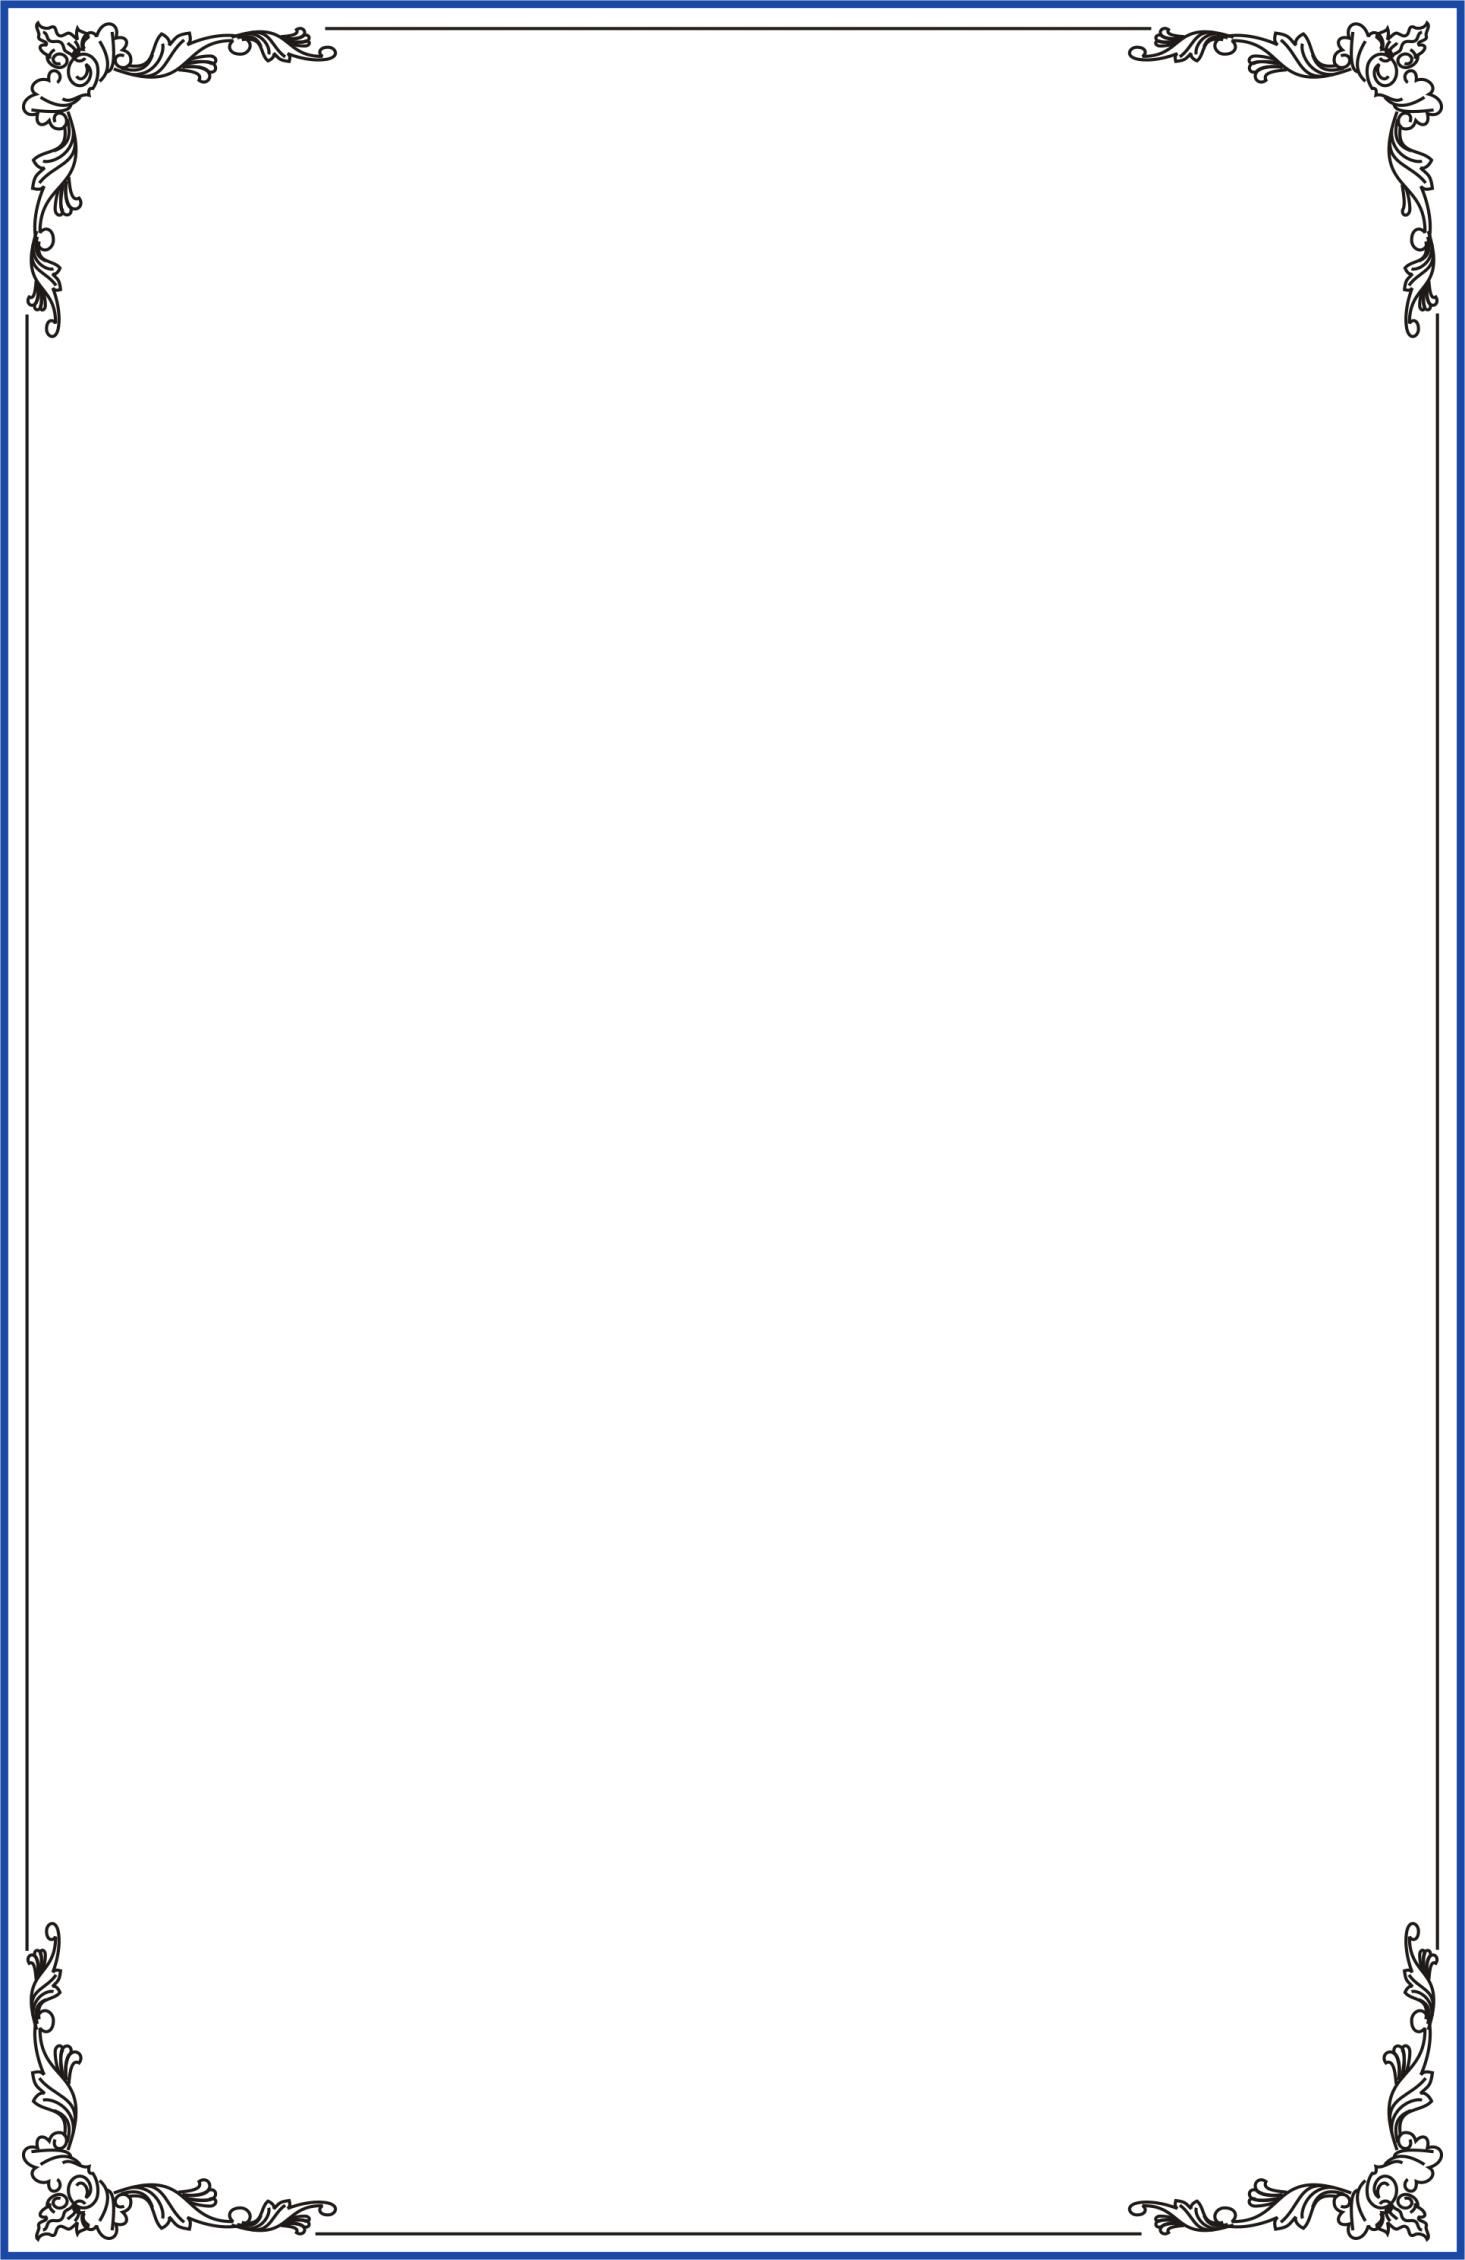
\includegraphics[width=17.2cm,height=26.5cm,keepaspectratio]{images/vien_bia_xanh.png}};
\end{tikzpicture}\par
\centering
{\bfseries ĐẠI HỌC THÁI NGUYÊN\par
TRƯỜNG ĐẠI HỌC CÔNG NGHỆ THÔNG TIN VÀ TRUYỀN THÔNG\par
KHOA CÔNG NGHỆ THÔNG TIN\par}
\vspace{1cm}

\includegraphics[width=3.5cm]{images/img01.png}\par
\vspace{1.5cm}
{\bfseries\Large BÁO CÁO DỰ ÁN\par}
{\bfseries\large HỌC PHẦN HỌC SÂU (DEEP LEARNING)\par}
\vspace{1.5cm}
{\bfseries Đề tài:\par}
\vspace{0.3cm}
{\bfseries\Large PHÁT HIỆN VÀ ĐỊNH VỊ BẤT THƯỜNG\\ TRÊN SẢN PHẨM CÔNG NGHIỆP\\ BẰNG HỌC KHÔNG GIÁM SÁT\par}
\vspace{1.5cm}
\begin{tabular}{@{}l l@{}}
\bfseries Tên nhóm: & \color{xanhbien}\bfseries NHÓM 13 \\[0.4cm]
\bfseries Sinh viên thực hiện: & \color{xanhbien}\bfseries Đặng Hoàng An \\
 & \color{xanhbien}\bfseries Trần Văn Dưỡng \\
 & \color{xanhbien}\bfseries Lớp KHMT K22A \\[0.4cm]
\bfseries Giáo viên hướng dẫn: & TS. Ngô Hữu Huy \\
\end{tabular}
\vfill
{\bfseries THÁI NGUYÊN, NĂM 2026\par}
\end{titlepage}
\restoregeometry


\pagenumbering{roman}
\tableofcontents
\clearpage
\listoffigures
\clearpage
\listoftables
\clearpage
\chapter*{PHÂN CÔNG NHIỆM VỤ}

\begin{table}[htbp]
  \centering
  \small
  \begin{tabular}{@{}>{\raggedright\arraybackslash}p{3.4cm} >{\raggedright\arraybackslash}p{11.2cm}@{}}
    \toprule
    Thành viên & Nhiệm vụ \\
    \midrule
    Đặng Hoàng An &
      Xây dựng và huấn luyện Autoencoder; chạy PatchCore trên 8 loại (bottle, cable, capsule, carpet, grid,
      hazelnut, leather, metal\_nut); demo; tài liệu hướng dẫn của kho mã nguồn. \\
    \addlinespace
    Trần Văn Dưỡng &
      Module đọc dữ liệu MVTec AD; module đánh giá (AUROC, hình minh họa, ghi kết quả); PaDiM; chạy PatchCore
      trên 7 loại (pill, screw, tile, toothbrush, transistor, wood, zipper). \\
    \addlinespace
    Cả nhóm &
      Cấu hình và giao thức đánh giá chung; tiện ích chạy Anomalib; tổng hợp kết quả; viết báo cáo. \\
    \bottomrule
  \end{tabular}
\end{table}

\clearpage
\pagenumbering{arabic}

\chapter*{MỞ ĐẦU}

Kiểm tra chất lượng là khâu bắt buộc trong sản xuất công nghiệp: sản phẩm có vết xước,
nứt, nhiễm bẩn hay thiếu chi tiết phải bị loại trước khi đến tay người dùng. Kiểm tra bằng mắt người chậm, phụ thuộc
kinh nghiệm và dễ bỏ sót khi sản lượng lớn hoặc lỗi nhỏ. Thị giác máy tính có thể tự động hóa khâu này, nhưng gặp một
khó khăn về dữ liệu: ảnh sản phẩm lỗi hiếm, đa dạng và khó lường trước, còn việc khoanh vùng lỗi trên từng ảnh để làm
nhãn tốn nhiều công sức, trong khi mô hình phân loại có giám sát chỉ nhận ra những kiểu lỗi đã thấy. Ngược lại, ảnh sản phẩm tốt có sẵn với số lượng lớn. Vì vậy, hướng học không giám sát, tức chỉ học từ ảnh tốt rồi
coi mọi sai khác đáng kể là bất thường, phù hợp hơn với điều kiện thực tế~\cite{bergmannMVTecADComprehensive2019}.

Đề tài xây dựng và đánh giá ba phương pháp phát hiện và định vị bất thường không giám sát trên
ảnh sản phẩm công nghiệp, nhằm trả lời ba câu hỏi: phương pháp nào phát hiện và khoanh vùng lỗi chính xác nhất;
phương pháp nào phù hợp với loại sản phẩm nào (bề mặt hay vật thể, vị trí cố định hay xoay); và mỗi phương pháp đánh
đổi giữa độ chính xác với thời gian, bộ nhớ ra sao.

Ba phương pháp được chọn đại diện cho hai hướng tiếp cận. Autoencoder, do nhóm tự xây
dựng, học tái tạo ảnh từ đầu và dùng sai số tái tạo làm tín hiệu bất thường.
PaDiM~\cite{defardPaDiMPatchDistribution2021} và PatchCore~\cite{rothTotalRecallIndustrial2022} dùng đặc trưng của
mạng tích chập đã học trước trên ImageNet, lần lượt mô hình hóa đặc trưng bình thường bằng phân phối Gauss theo vị
trí và bằng một bộ nhớ các vector đặc trưng. Dữ liệu là đủ 15 loại sản phẩm của bộ MVTec
AD~\cite{bergmannMVTecADComprehensive2019}. Đề tài dừng ở mức đánh giá trên dữ liệu ảnh có sẵn, chưa triển khai trên
dây chuyền và chưa chọn ngưỡng quyết định cho sử dụng thực tế.

Về cách làm, nhóm tìm hiểu cơ chế của từng phương pháp qua bài báo gốc, cài đặt chúng theo cùng
một giao thức, chạy trên cả 15 loại và đánh giá bằng
image-AUROC cho nhiệm vụ phát hiện ảnh lỗi, pixel-AUROC cho nhiệm vụ định vị vùng lỗi.
Kết quả cho thấy PatchCore đạt image-AUROC trung bình 0,983 và pixel-AUROC 0,980, sát số liệu công bố; PaDiM
đạt 0,890 và 0,960 với thời gian xây dựng mô hình ngắn nhất; Autoencoder đạt 0,756 và 0,843. Như vậy, với
vài trăm ảnh tốt cho mỗi loại, dùng lại đặc trưng học trước hiệu quả hơn nhiều so với học tái tạo ảnh từ đầu.

Chương 1 trình bày cơ sở lý thuyết: học sâu, mạng tích chập, đặc trưng học trước, bài toán
phát hiện bất thường và cách đánh giá. Chương 2 trình bày bộ dữ liệu, giao thức đánh giá và cách triển khai ba
phương pháp. Chương 3 trình bày kết quả thực nghiệm và đánh giá.

\chapter{CƠ SỞ LÝ THUYẾT}

\section{Tìm hiểu về Trí tuệ nhân tạo, Học máy, Học sâu}

\subsection{Trí tuệ nhân tạo (Artificial Intelligence - AI)}

Trí tuệ nhân tạo (AI) là một lĩnh vực khoa học tập trung vào việc xây dựng và cải tiến các hệ thống tính toán tự động có thể đảm nhiệm những công việc vốn đòi hỏi trí tuệ của con người. Công nghệ này mô phỏng các quá trình tư duy, học hỏi và giải quyết vấn đề, với mục tiêu xây dựng những hệ thống có khả năng nhận thức, suy nghĩ và hành động một cách tự động.

AI bao gồm nhiều kỹ thuật và phương pháp đa dạng như Học máy (Machine Learning), Xử lý ngôn ngữ tự nhiên (Natural Language Processing) và Thị giác máy tính (Computer Vision). Các tiến bộ kỹ thuật gần đây đóng vai trò then chốt trong việc hiện thực hóa các hệ thống AI hiệu quả và đáng tin cậy cho phép máy tính tiếp thu kiến thức từ dữ liệu, nhận diện các mẫu đặc trưng, thích ứng với hoàn cảnh mới và đưa ra các quyết định một cách thông minh. AI có thể được phân loại thành ba cấp độ:
\begin{itemize}
  \item AI yếu (Narrow AI): AI được phát triển để thực hiện một tác vụ đơn giản, cụ thể, ví dụ như chatbot, hệ thống đề xuất phim, hoặc trợ lý ảo.
  \item AI mạnh (General AI): Có khả năng học và thực hiện bất kỳ nhiệm vụ trí tuệ nào của con người.
  \item AI siêu việt (Super AI): Là giai đoạn lý thuyết trong tương lai, nơi AI có thể vượt xa trí thông minh của con người trong mọi lĩnh vực.
\end{itemize}

Trong thời đại số hóa hiện nay, trí tuệ nhân tạo (AI) ngày càng trở thành yếu tố cốt lõi thúc đẩy sự đổi mới và phát triển trong các ngành như chăm sóc sức khỏe, tài chính, vận tải và ngành công nghiệp giải trí, mang lại những đổi mới đáng kể trong cách chúng ta học tập và làm việc.

\subsection{Học máy (Machine Learning - ML)}

Học máy (Machine Learning) là một phân ngành của Trí tuệ nhân tạo (AI) chuyên nghiên cứu các thuật toán giúp hệ thống học từ dữ liệu và đưa ra quyết định mà không cần mã hóa quy tắc một cách rõ ràng.

Nguyên lý hoạt động của ML dựa trên việc rút ra mô hình từ dữ liệu huấn luyện (training data) để đưa ra dự đoán hoặc quyết định cho dữ liệu mới (dữ liệu kiểm tra).

Học máy bao gồm ba nhóm chính dựa trên cách mô tả tiếp cận dữ liệu:
\begin{itemize}
  \item Học có giám sát (Supervised Learning): Phương pháp này sử dụng tập dữ liệu đã được gán nhãn sẵn để huấn luyện mô hình. Ví dụ việc phân loại thư rác.
  \item Học không giám sát (Unsupervised Learning): Với phương pháp này, hệ thống làm việc với dữ liệu không có nhãn, nhiệm vụ của mô hình là tìm ra những đặc điểm hoặc mối quan hệ tiềm ẩn bên trong. Ví dụ: phân loại người dùng mạng xã hội theo hành vi tương tác.
  \item Học tăng cường (Reinforcement Learning): Dựa trên quá trình tương tác giữa hệ thống và môi trường, trong đó hệ thống nhận được phần thưởng khi thực hiện hành vi đúng. Một minh họa rõ nét là robot học cách di chuyển nhờ việc liên tục thử các ra quyết định và điều chỉnh dựa trên phản hồi môi trường mang lại.
\end{itemize}

\begin{figure}[htbp]
  \centering
  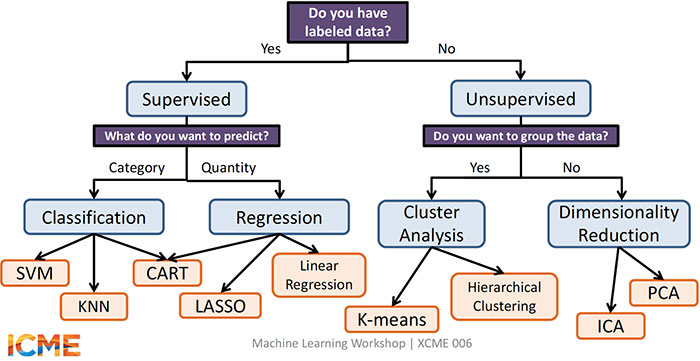
\includegraphics[width=0.8\linewidth]{images/img02.jpeg}
  \caption{Các thuật toán Học máy}
  \label{fig:ml-algorithms}
\end{figure}

\subsection{Học sâu (Deep Learning - DL)}

Học sâu (Deep Learning) là một lĩnh vực trực thuộc học máy, sử dụng các mạng nơ-ron nhiều tầng để xây dựng mô hình toán học dựa trên dữ liệu đầu vào. Deep Learning thường được nhắc đến song song với Trí tuệ nhân tạo (AI) và Dữ liệu lớn (Big Data). Công nghệ này đã được áp dụng và hiện vẫn tiếp tục được ứng dụng rộng rãi trong thực tế, được thúc đẩy mạnh mẽ bởi sự tiến hóa của phần cứng, nhờ vào sức mạnh xử lý của GPU, lượng dữ liệu tăng nhanh, cùng với sự hỗ trợ từ các thư viện như TensorFlow và PyTorch, việc phát triển mô hình đã được đơn giản hóa, giúp cho người dùng dễ dàng thao tác sử dụng hơn.

Học sâu khai thác khả năng học biểu diễn đặc trưng trực tiếp từ dữ liệu. Một quan sát cụ thể, ví dụ hình ảnh, có khả năng được bằng nhiều hình thức khác nhau – từ các vector chứa giá trị điểm ảnh đến các biểu diễn trừu tượng như tập hợp cạnh, vùng hoặc hình khối. Ví dụ minh họa bao gồm nhận diện khuôn mặt hoặc phân tích biểu cảm khuôn mặt. Một điểm mạnh đáng chú ý của học sâu là khả năng loại bỏ các đặc trưng thủ công và thay vào đó là các đặc trưng trích xuất tự động thông qua quá trình học, đặc biệt hiệu quả trong các bài toán học không giám sát (unsupervised learning) và bán giám sát (semi-supervised learning) nhờ vào cấu trúc phân cấp.

Các kiến trúc học sâu tiêu biểu như mạng nơ-ron sâu (Deep Neural Networks - DNN), mạng tích chập (Convolutional Neural Networks - CNN), mạng niềm tin sâu (Deep Belief Networks - DBN) và mạng hồi tiếp (Recurrent Neural Networks - RNN) đã được triển khai rộng rãi trong nhiều lĩnh vực, bao gồm nhận dạng hình ảnh, phân tích giọng nói, xử lý văn bản tự nhiên, âm thanh và sinh học tính toán. Những mô hình này đã chứng minh hiệu quả vượt trội khi giải quyết các tác vụ phức tạp trong thực tiễn.

Thêm vào đó, học sâu hiện nay cũng trở thành một thuật ngữ phổ biến, đôi khi được xem như "thương hiệu" đại diện cho các mạng nơ-ron sâu hiện đại (modern deep neural network).

\begin{figure}[htbp]
  \centering
  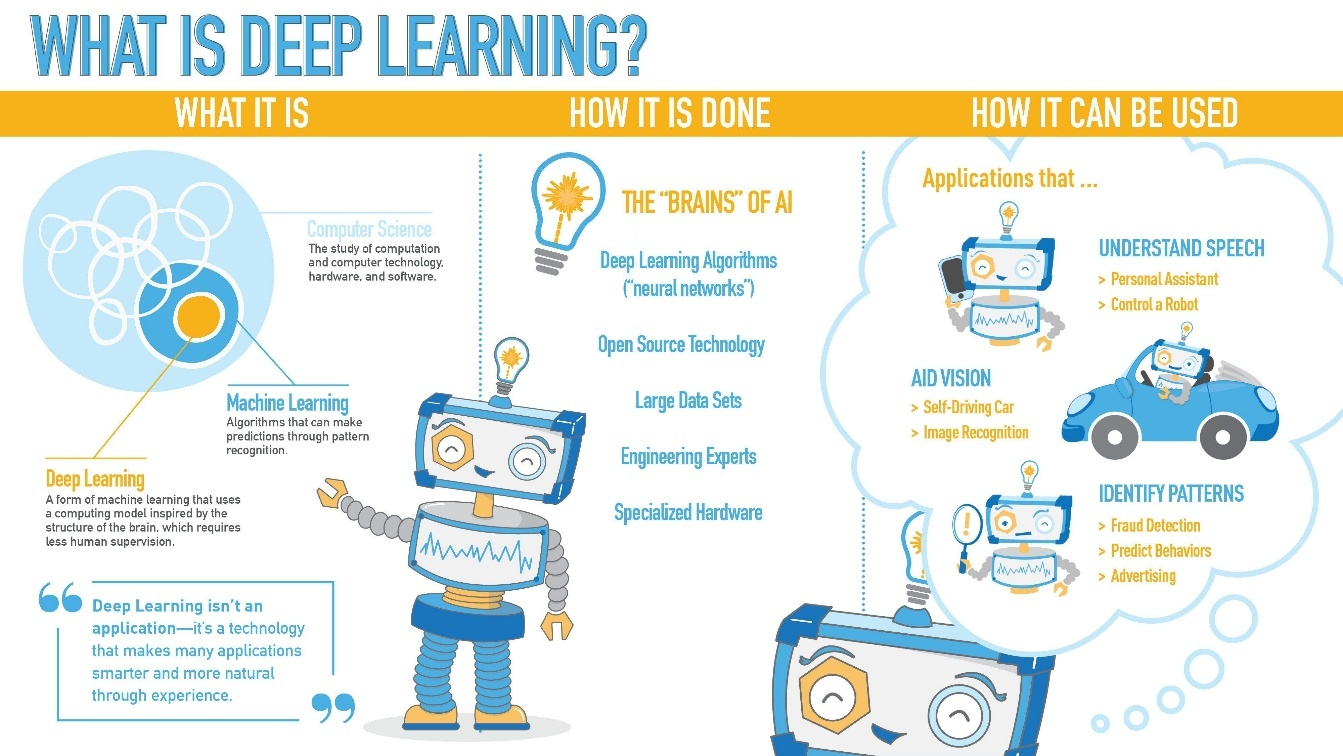
\includegraphics[width=0.8\linewidth]{images/img03.jpeg}
  \caption{Học sâu}
  \label{fig:deep-learning}
\end{figure}

\subsection{Mối quan hệ giữa trí Tuệ nhân tạo, Học máy, Học sâu}

Trí tuệ nhân tạo (Artificial Intelligence – AI), Học máy (Machine Learning – ML) và Học sâu (Deep Learning – DL) là ba khái niệm có mối quan hệ mật thiết với nhau, đồng thời phản ánh tiến trình phát triển tự nhiên của lĩnh vực nghiên cứu về khả năng tiếp nhận kiến thức và tư duy của máy móc.

Trí tuệ nhân tạo là lĩnh vực tổng quát, bao gồm tất cả các phương pháp và kỹ thuật nhằm mục đích tạo ra các hệ thống có khả năng thực hiện các hành vi thông minh tương tự con người. Trong phạm vi này, học máy xuất hiện như một hướng tiếp cận nổi bật, tập trung vào việc xây dựng các kỹ thuật cho phép máy tính có thể học được thông qua dữ liệu mà không cần phải lập trình tường minh cho từng tác vụ cụ thể. Học máy không chỉ giúp tự động hóa quá trình ra quyết định mà còn mở ra khả năng xử lý các vấn đề phức tạp trong môi trường có dữ liệu thay đổi liên tục.

Tiếp nối sự phát triển của học máy, học sâu được xem là một phân nhánh sâu hơn, sử dụng mô hình hệ thống mạng nơ-ron đa tầng (deep neural networks) để mô hình hóa các quan hệ phi tuyến phức tạp giữa dữ liệu đầu vào và đầu ra. Học sâu cho phép khai thác dữ liệu ở quy mô lớn và có khả năng trích xuất đặc trưng tự động, thay vì dựa vào đặc trưng thủ công như trong các phương pháp học máy truyền thống.

Giữa ba lĩnh vực này có mối quan gắn bó chặt chẽ với nhau, được tổ chức theo mô hình lồng ghép – trong đó mỗi lĩnh vực là nền tảng cho lĩnh vực tiếp theo, trong đó học sâu là một phần của học máy, và học máy là một phần của trí tuệ nhân tạo. Cụ thể: Deep Learning $\subset$ Machine Learning $\subset$ Artificial Intelligence. Đây không những là mối quan hệ phân lớp mà còn là sự kế thừa và nâng cao về mặt kỹ thuật và ứng dụng.

\begin{figure}[htbp]
  \centering
  
\includegraphics[width=0.8\linewidth]{images/img04.jpeg}
  \caption{Mối quan hệ giữa trí tuệ nhân tạo, học máy, học sâu}
  \label{fig:ai-ml-dl}
\end{figure}

\section{Các thành phần cơ bản trong hệ thống học máy và học sâu}

\subsection{Dữ liệu trong học máy và học sâu}

Dữ liệu là yếu tố cốt lõi trong suốt quá trình đào tạo mô hình học máy và học sâu. Chất lượng và số lượng dữ liệu ảnh hưởng trực tiếp đến độ tin cậy và khả năng mở rộng của mô hình.

Phân loại dữ liệu:
\begin{itemize}
  \item Dữ liệu có cấu trúc (Structured data): Dữ liệu dạng bảng, có trường và giá trị rõ ràng, như cơ sở dữ liệu SQL.
  \item Dữ liệu phi cấu trúc (Unstructured data): Hình ảnh, video, âm thanh, văn bản...
  \item Dữ liệu bán cấu trúc (Semi-structured data): JSON, XML hoặc log hệ thống.
\end{itemize}

Tiền xử lý dữ liệu (Data Preprocessing): Là bước quan trọng để loại bỏ nhiễu, chuẩn hóa đầu vào, và tăng độ chính xác cho mô hình. Bao gồm:
\begin{itemize}
  \item Làm sạch dữ liệu (loại bỏ nhiễu trong tập dữ liệu thông qua việc xử lý thiếu hụt thông tin và phát hiện ngoại lệ),
  \item Chuẩn hóa (Normalization, Standardization),
  \item Mã hóa dữ liệu (One-hot, Label encoding),
  \item Chia tập dữ liệu (train/test/validation),
  \item Tăng cường dữ liệu (Data Augmentation – với hình ảnh hoặc âm thanh).
\end{itemize}

\subsection{Kiến trúc mạng nơ-ron nhân tạo}

Mạng nơ-ron nhân tạo (ANN) là thành phần chính trong học sâu. Cấu trúc cơ bản của một mạng gồm ba lớp~\cite{zhangMultilayerPerceptrons}:
\begin{itemize}
  \item Lớp đầu vào (Input layer): Nhận dữ liệu thô từ bên ngoài.
  \item Lớp ẩn (Hidden layer): Thực hiện các phép toán, phát hiện đặc trưng.
  \item Lớp đầu ra (Output layer): Trả kết quả dự đoán cuối cùng.
\end{itemize}

Các nơ-ron trong từng lớp được kết nối với các nơ-ron ở lớp kế tiếp thông qua trọng số. Việc sử dụng nhiều lớp ẩn trong các mạng học sâu giúp mô hình học được những đặc trưng dữ liệu ở mức độ trừu tượng cao hơn.

\begin{figure}[htbp]
  \centering
  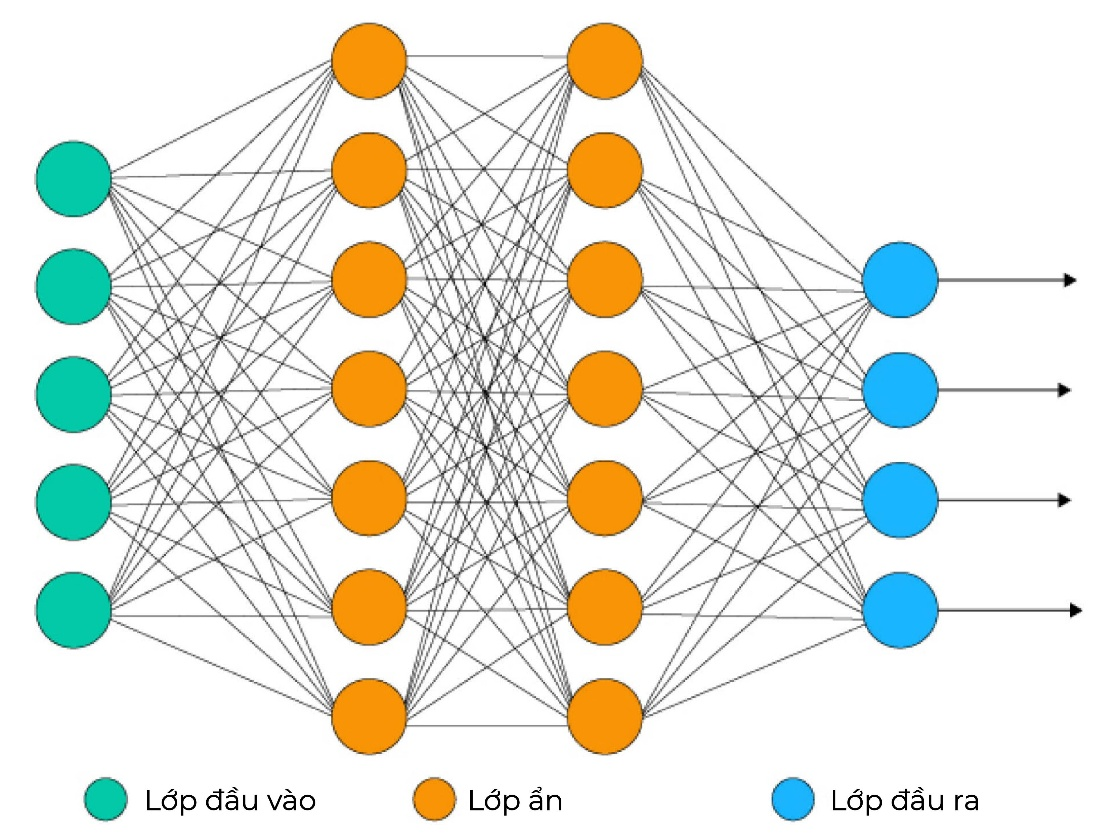
\includegraphics[width=0.8\linewidth]{images/img05.jpeg}
  \caption{Cấu trúc mạng nơ-ron nhân tạo}
  \label{fig:ann}
\end{figure}

Một số kiến trúc đặc biệt:
\begin{itemize}
  \item CNN (Mạng tích chập): Xử lý ảnh và nhận diện không gian.
  \item RNN và LSTM: Phù hợp với dữ liệu chuỗi (speech, text).
  \item Transformer: Mô hình học ngữ cảnh sâu và xử lý song song trong NLP.
  \item Autoencoder: Dùng để giảm chiều dữ liệu, trích xuất đặc trưng.
\end{itemize}

\subsection{Quá trình huấn luyện mô hình}

Huấn luyện mô hình là quá trình tối ưu trọng số sao cho độ lệch giữa kết quả mô hình dự đoán và giá trị thực tế là nhỏ nhất~\cite{pytorchOptimizingModelParameters}. Gồm các bước:
\begin{enumerate}
  \item Khởi tạo trọng số (Weight Initialization)
  \item Lan truyền tiến (Forward Propagation)
  \item Tính toán sai số (Loss Function): Các hàm như MSE, Cross-Entropy.
  \item Lan truyền ngược (Backpropagation): Cập nhật trọng số theo hướng giảm sai số.
  \item Tối ưu hóa (Optimization): Dùng các thuật toán như SGD, Adam, RMSProp.
  \item Chống overfitting~\cite{zhangGeneralization}: Dropout, Regularization (L1/L2), Early Stopping, v.v.
\end{enumerate}

\subsection{Đánh giá mô hình}

Quy trình đánh giá mô hình giúp xác định độ chính xác và tính tổng quát hóa~\cite{zhangGeneralization}. Một số chỉ số phổ biến:
\begin{itemize}
  \item Độ chính xác (Accuracy)
  \item Precision / Recall / F1-Score
  \item AUC-ROC (cho mô hình phân loại)
  \item MAE, RMSE (cho bài toán hồi quy)
\end{itemize}
Công cụ hỗ trợ đánh giá: confusion matrix, learning curve, validation curve,\ldots

\subsection{Các công cụ và thư viện hỗ trợ}

Triển khai các giải pháp dựa trên học máy và học sâu hiện nay được hỗ trợ bởi rất nhiều thư viện mã nguồn mở mạnh mẽ~\cite{tensorflowTensorFlow,pytorchOptimizingModelParameters,scikit-learnMachineLearning,numpyNumPy,matplotlibVisualizationPython}:

\begin{table}[htbp]
  \centering
  \caption{Các công cụ, thư viện hỗ trợ}
  \label{tab:tools}
  \begin{tabular}{@{}l l l@{}}
    \toprule
    Công cụ/Thư viện & Mục đích & Ngôn ngữ \\
    \midrule
    TensorFlow & Học sâu, hỗ trợ GPU, mô hình hóa linh hoạt & Python, C++ \\
    Keras & API cấp cao của TensorFlow, dễ dùng & Python \\
    PyTorch & Mạnh mẽ và linh hoạt, phổ biến trong nghiên cứu & Python \\
    OpenCV & Xử lý ảnh, phát hiện đối tượng & Python, C++ \\
    Pandas, NumPy & Xử lý dữ liệu & Python \\
    \bottomrule
  \end{tabular}
\end{table}

\section{Ứng dụng của trí tuệ nhân tạo, học máy và học sâu}

Cùng với sự phát triển nhanh chóng của phần cứng và dữ liệu lớn (Big Data), AI, học máy và học sâu đã và đang được ứng dụng mạnh mẽ trong nhiều ngành nghề, góp phần nâng cao năng suất, tối ưu hóa vận hành, và đóng góp vào việc tạo dựng giá trị thiết thực cho doanh nghiệp cũng như xã hội.

\subsection{Thị giác máy tính (Computer Vision)}

Thị giác máy tính là một trong những lĩnh vực cốt lõi của trí tuệ nhân tạo, cho phép máy móc có khả năng nhận diện và hiểu biết về môi trường xung quanh qua các hình ảnh hoặc đoạn video. Công nghệ này sử dụng ứng dụng các phương pháp học máy, trong đó học sâu đóng vai trò then chốt, vốn nổi bật trong việc xử lý các hình ảnh có cấu trúc phức tạp và đa dạng về đặc trưng.

Một trong những ứng dụng rộng rãi là hệ thống nhận dạng khuôn mặt, sử dụng mạng nơ-ron tích chập (CNN) để phân tích các đặc trưng khuôn mặt, áp dụng rộng rãi trong mở khóa thiết bị di động, hệ thống giám sát an ninh, hay quản lý điểm danh thông minh.

Trong lĩnh vực y tế, học sâu được dùng để phân loại hình ảnh y học như ảnh CT, MRI, X-quang nhằm phát hiện bệnh lý như ung thư, xuất huyết hoặc tổn thương mô mềm. Các hệ thống này không chỉ hỗ trợ bác sĩ mà còn nâng cao độ chính xác chẩn đoán nhờ khả năng học từ hàng triệu mẫu ảnh.

Công nghệ phát hiện và theo dõi đối tượng cũng là một bước tiến lớn, ứng dụng trong xe tự hành và các hệ thống giám sát giao thông thông minh. Thuật toán như YOLO, SSD hay Mask R-CNN có khả năng nhận diện nhiều đối tượng trong thời gian thực, hỗ trợ các hệ thống đưa ra quyết định điều hướng và phản ứng kịp thời.

Thị giác máy tính cũng góp phần trong việc số hóa tài liệu thông qua công nghệ nhận diện ký tự quang học (OCR), giúp máy đọc được văn bản từ ảnh chụp, hóa đơn hoặc tài liệu scan, hỗ trợ hiệu quả trong lưu trữ và tìm kiếm thông tin.

Ngoài ra, trong lĩnh vực sáng tạo và giải trí, thị giác máy tính được tích hợp công nghệ AR vào việc xử lý và áp dụng hiệu ứng khuôn mặt trực tiếp, hiệu ứng video, hoặc thậm chí trong các công cụ tạo nghệ thuật số nhờ khả năng hiểu cấu trúc và thành phần hình ảnh.

\begin{figure}[htbp]
  \centering
  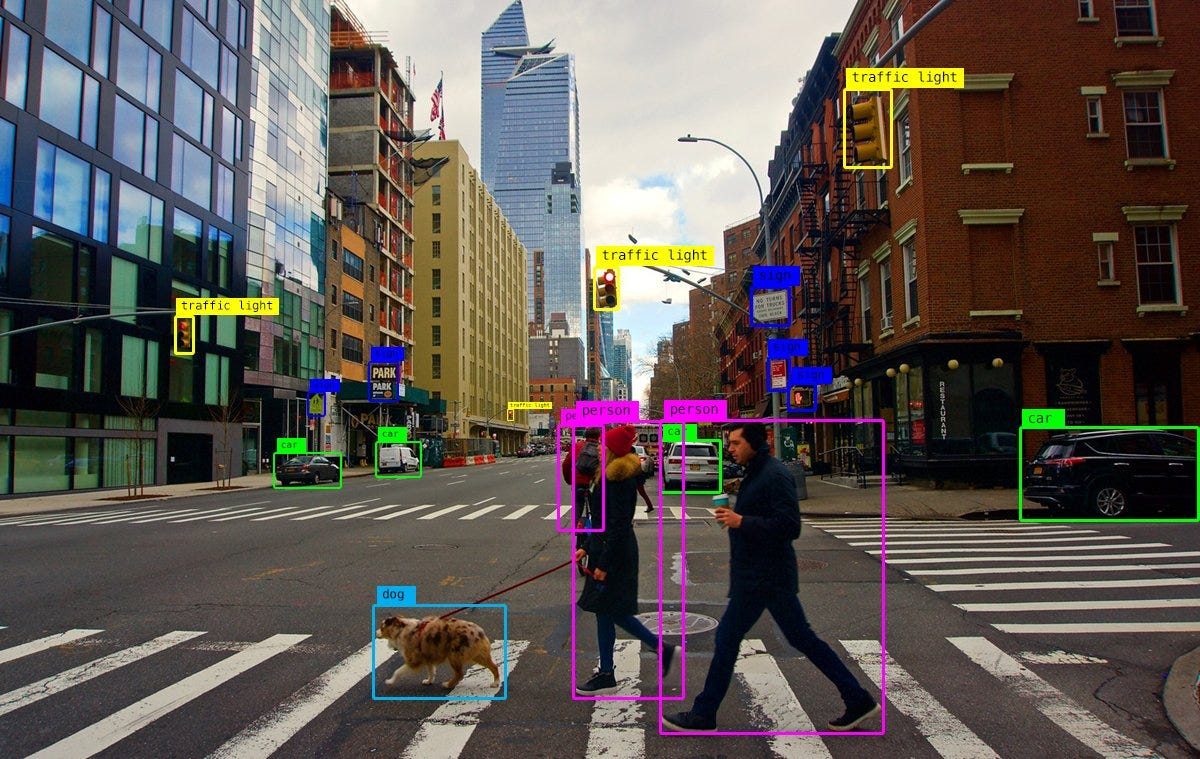
\includegraphics[width=0.8\linewidth]{images/img06.jpg}
  \caption{Ứng dụng của Thị giác máy tính trong nhận diện vật thể}
  \label{fig:cv-detection}
\end{figure}

\subsection{Xử lý ngôn ngữ tự nhiên (Natural Language Processing - NLP)}

Xử lý ngôn ngữ tự nhiên là một lĩnh vực nghiên cứu nhằm trang bị cho máy tính khả năng hiểu, phân tích và sinh ngôn ngữ tự nhiên theo cách mà con người sử dụng trong giao tiếp. Đây là một trong những hướng phát triển sôi động nhất của AI hiện đại, với sự bùng nổ mạnh mẽ của các mô hình học sâu như BERT, GPT, T5 và các mô hình ngôn ngữ lớn (LLMs).

Một trong những ví dụ điển hình nhất của NLP là chatbot và trợ lý ảo – như Siri, Alexa, Google Assistant – cho phép máy có thể hiểu các yêu cầu bằng giọng nói hoặc văn bản và phản hồi một cách tự nhiên. Học sâu đóng vai trò quan trọng trong việc tạo ra phản hồi mạch lạc, đúng ngữ cảnh và có khả năng cá nhân hóa cao.

Dịch máy tự động cũng đã có bước tiến vượt bậc. Các mô hình học sâu tiên tiến như Transformer đã mở ra nhiều hướng tiếp cận hiệu quả, hệ thống như Google Translate hay DeepL không chỉ dịch chính xác hơn mà còn giữ được ngữ điệu và phong cách văn bản gốc.

Phân tích cảm xúc là một ứng dụng khác, sử dụng NLP để đánh giá tâm trạng hoặc thái độ của người dùng dựa trên nội dung văn bản – rất hữu ích trong phân tích đánh giá sản phẩm, phản hồi khách hàng hoặc theo dõi dư luận trên mạng xã hội.

Trong lĩnh vực tóm tắt văn bản, các mô hình hiện đại có thể tự động rút gọn nội dung từ bài viết, tài liệu dài thành bản tóm tắt ngắn gọn, vẫn đảm bảo thông tin cốt lõi, phục vụ cho nghiên cứu, báo cáo hay tổng hợp tin tức.

Ngoài ra, NLP hỗ trợ nhận diện các thực thể tên riêng thông qua kỹ thuật NER, cho phép trích xuất thông tin quan trọng như tên người, địa điểm, tổ chức từ văn bản – một phương pháp hiệu quả trong lĩnh vực phân tích dữ liệu văn bản và xây dựng cơ sở tri thức.

Nhờ sự phát triển đồng bộ của AI, học máy và học sâu, NLP ngày càng trở nên mạnh mẽ, không chỉ giúp máy hiểu ngôn ngữ con người mà còn có khả năng tham gia đối thoại tự nhiên, sinh văn bản sáng tạo và hỗ trợ nhiều tác vụ trí tuệ phức tạp.

\begin{figure}[htbp]
  \centering
  
\includegraphics[width=0.8\linewidth]{images/img07.png}
  \caption{Chatbot – Ứng dụng của xử lý ngôn ngữ tự nhiên}
  \label{fig:chatbot}
\end{figure}

\subsection{Xử lý ảnh}

Xử lý ảnh là một trong những bài toán nền tảng trong trí tuệ nhân tạo, học máy và học sâu, với mục tiêu chính là phân tích, trích xuất thông tin từ hình ảnh hoặc thực hiện các phép biến đổi nhằm phục vụ cho những tác vụ cao hơn như nhận diện, theo dõi, hoặc ra quyết định.

Một ứng dụng quen thuộc là gắn thẻ hình ảnh (image tagging), chẳng hạn như khi người dùng đăng ảnh lên mạng xã hội, thuật toán có khả năng nhận diện tự động và đề xuất thẻ tên cho khuôn mặt xuất hiện trong ảnh. Cơ chế đằng sau đó thường dựa vào các mô hình học sâu, trong đó mạng nơ-ron CNN được sử dụng phổ biến nhất, có khả năng học từ dữ liệu gắn nhãn sẵn (ảnh người dùng từng được gắn thẻ trước đó), từ đó nhận diện lại trong các bức ảnh mới.

Một ứng dụng khác là nhận dạng ký tự quang học (OCR – Optical Character Recognition), cho phép chuyển đổi hình ảnh chứa văn bản thành dữ liệu số có thể chỉnh sửa và tìm kiếm. Các mô hình học máy và học sâu được phát triển nhằm mục đích nhận dạng các ký tự xuất hiện trong hình ảnh, bất kể font chữ, bố cục hay chất lượng hình ảnh, từ đó phục vụ cho số hóa tài liệu, trích xuất thông tin trên hóa đơn, văn bản hành chính\ldots

Trong lĩnh vực phương tiện tự hành, xử lý ảnh đóng vai trò như “đôi mắt” của hệ thống điều khiển. Thuật toán học máy và học sâu liên tục xử lý các khung hình thu được từ camera gắn trên xe, giúp phát hiện mép đường, biển báo, làn xe, người đi bộ và các vật cản. Đây là tiền đề để xe đưa ra hành động như rẽ, phanh hay tăng tốc một cách chính xác và an toàn.

\subsection{Y tế và chăm sóc sức khỏe}

Trong lĩnh vực y tế, trí tuệ nhân tạo đóng vai trò quan trọng trong việc hỗ trợ bác sĩ chẩn đoán và ra quyết định điều trị. Học máy được áp dụng để nghiên cứu trong hồ sơ bệnh án số (EHR), từ đó phát hiện sớm nguy cơ mắc bệnh như tiểu đường, tim mạch, hoặc tái phát ung thư. Học sâu trong xử lý hình ảnh y tế còn đặc biệt hiệu quả như X-quang, CT hay MRI góp phần hỗ trợ phát hiện sớm tổn thương, khối u với độ chính xác cao hơn cả một số chuyên gia trong từng tình huống cụ thể.

Ngoài ra, các thuật toán AI còn góp phần thúc đẩy quá trình nghiên cứu và phát triển dược phẩm, mô phỏng phản ứng phân tử và tối ưu hiệu năng thử nghiệm lâm sàng. Các hệ thống khuyến nghị điều trị, kết hợp dữ liệu bệnh nhân và hướng dẫn y khoa, là sự tổng hòa giữa AI truyền thống và các mô hình học máy hiện đại.

\subsection{Tài chính – ngân hàng}

AI, ML và DL đang làm thay đổi sâu sắc ngành tài chính. Các mô hình học máy hỗ trợ quy trình chấm điểm tín dụng, tự động hóa quy trình phân tích rủi ro tiềm ẩn cùng với nhận dạng các hành vi lừa đảo trong giao dịch tài chính nhờ vào việc học từ dữ liệu lịch sử. Học sâu còn được triển khai trong việc phân tích chuỗi thời gian phức tạp như biến động thị trường chứng khoán hoặc hành vi khách hàng đa kênh.

Ngoài ra, các tổ chức tài chính, bao gồm ngân hàng đã ứng dụng chatbot thông minh dựa trên học sâu để cung cấp tư vấn tài chính cá nhân hóa, giúp cải thiện trải nghiệm khách hàng và giảm tải cho tổng đài viên. Từ đó, AI không chỉ hỗ trợ tự động hóa, mà còn tạo ra lợi thế cạnh tranh vượt trội trong thị trường tài chính hiện đại.

\subsection{Giao thông và phương tiện tự hành}

Phương tiện tự lái là một minh chứng rõ ràng cho việc triển khai sâu rộng các giải pháp trí tuệ nhân tạo trong thực tiễn của cả AI, ML và DL. AI giúp hệ thống đưa ra quyết định tổng thể, trong khi ML học từ hành vi lái xe để tối ưu hoá hành động, và DL xử lý trực tiếp tín hiệu đầu vào từ camera, radar, LiDAR để nhận diện đường đi, vật cản, biển báo hoạt động theo thời gian thực.

Giải pháp quản lý giao thông hiện đại và thông minh dựa trên bản đồ số cũng ứng dụng học máy nhằm xử lý và khai thác dữ liệu lớn trong thời gian thực, từ đó hỗ trợ quá trình ra quyết định hiệu quả hơn, tối ưu hóa lộ trình. Ở cấp đô thị, AI giúp phân tích dòng xe, dự báo mật độ giao thông, điều phối đèn tín hiệu một cách thích ứng, góp phần giảm tắc nghẽn và tai nạn.

\subsection{Công nghiệp và sản xuất}

Trong công nghiệp, AI giúp cải thiện hiệu suất và giảm thiểu lãng phí thông qua các hệ thống ra quyết định thông minh. Học máy được ứng dụng trong bảo trì dự đoán – nơi các mô hình học từ dữ liệu cảm biến để dự báo tình trạng máy móc, tránh hỏng hóc đột xuất. Học sâu hỗ trợ thị giác máy tính trong dây chuyền kiểm tra chất lượng tự động hóa, giúp hệ thống phát hiện lỗi sản phẩm với tốc độ và độ chính xác cao.

Ngoài ra, robot cộng tác (cobots) – thường được điều khiển bởi hệ thống học sâu – có khả năng học hỏi từ hành vi con người và làm việc linh hoạt trong môi trường sản xuất hỗn hợp. Việc tối ưu chuỗi cung ứng cũng dựa vào các mô hình học máy để phân tích xu hướng tiêu dùng, dự báo nhu cầu và quản lý kho hiệu quả hơn.

\subsection{Giáo dục và đào tạo}

AI hỗ trợ cá nhân hóa quá trình học tập bằng cách đề xuất nội dung phù hợp với trình độ và sở thích của từng học sinh. Học máy được ứng dụng trong việc nghiên cứu hành vi học tập và dự đoán nguy cơ bỏ học hoặc tụt lùi trong quá trình học, từ đó hỗ trợ giảng viên đưa ra các can thiệp kịp thời.

Học sâu giữ vai trò thiết yếu trong việc xây dựng các hệ thống chấm điểm tự động, đặc biệt là với bài tập lập trình hoặc xử lý ngôn ngữ tự nhiên. Thêm vào đó, công nghệ thực tế ảo (VR/AR) kết hợp với AI mở ra các mô hình đào tạo mới, mô phỏng tình huống phức tạp như thí nghiệm hóa học, mô phỏng phòng mổ hay huấn luyện kỹ năng mềm.

\section{Tiểu kết chương 1}

Trong chương này, chúng ta đã cùng nhau tìm hiểu tổng quan về ba lĩnh vực công nghệ nổi bật và có ảnh hưởng lớn trong kỷ nguyên số hiện nay là trí tuệ nhân tạo (AI), học máy (Machine Learning) và học sâu (Deep Learning). Trong đó, AI là khái niệm tổng thể, còn học máy và học sâu đóng vai trò là những phương pháp then chốt trong việc phát triển các hệ thống thông minh giúp cho máy tính khai thác dữ liệu để tự động rút ra kết luận và có khả năng tự đưa ra quyết định dựa trên dữ liệu đầu vào mà không phụ thuộc vào các quy tắc được lập trình sẵn.

Chương còn đi sâu tìm hiểu các yếu tố thiết yếu trong một hệ thống học máy, bắt đầu từ dữ liệu đầu vào, mô hình mạng nơ-ron nhân tạo, quy trình huấn luyện và đánh giá mô hình, cùng với các công cụ hỗ trợ phổ biến như TensorFlow, PyTorch, Scikit-learn,\ldots Những kiến thức này đóng vai trò nền tảng trong việc phát triển các hệ thống thông minh ứng dụng trong thực tế.

Ngoài ra, chương cũng trình bày một số ứng dụng tiêu biểu của AI và học sâu trong nhiều lĩnh vực khác nhau. Những ví dụ này cho thấy rõ ràng tính thực tiễn cũng như tác động mạnh mẽ của các công nghệ đối với cuộc sống của con người.

Những nội dung đã giới thiệu trong chương 1 sẽ là cơ sở lý thuyết quan trọng, hỗ trợ cho việc khai thác sâu hơn ở các chương sau, nơi chúng ta nhắm đến mục tiêu giải quyết bài toán đặc thù mà đề tài hướng đến, lựa chọn mô hình học sâu phù hợp, cũng như các bước triển khai, huấn luyện và đánh giá mô hình trong thực tiễn.

\chapter{MÔ HÌNH HỌC SÂU TRONG PHÁT HIỆN BẤT THƯỜNG}

\section{Giới thiệu bài toán}

Trong kiểm tra chất lượng sản phẩm công nghiệp, các lỗi như vết xước, nứt, biến dạng hoặc thiếu chi tiết có thể xuất hiện với hình dạng và kích thước khác nhau. Việc kiểm tra thủ công phụ thuộc vào kinh nghiệm và khả năng quan sát của người thực hiện. Một hệ thống phân tích ảnh có thể hỗ trợ phát hiện dấu hiệu bất thường và chỉ ra vị trí cần kiểm tra, từ đó giúp quá trình đánh giá chất lượng có thêm căn cứ trực quan.

Khó khăn của bài toán nằm ở sự chênh lệch giữa dữ liệu bình thường và dữ liệu lỗi. Ảnh sản phẩm đạt yêu cầu thường dễ thu thập hơn, trong khi một số dạng lỗi ít xuất hiện hoặc chưa từng được ghi nhận. Nếu xây dựng bộ phân loại có giám sát cho từng loại lỗi, tập huấn luyện phải có đủ ví dụ đại diện của các lỗi đó. Điều kiện này khó đáp ứng khi lỗi mới tiếp tục phát sinh trong quá trình sản xuất.

Đề tài của nhóm 13 nghiên cứu hướng học đặc điểm của sản phẩm bình thường rồi đánh giá mức độ khác biệt của ảnh mới. Tập huấn luyện chỉ sử dụng ảnh tốt; ảnh lỗi và mặt nạ vùng lỗi được dùng ở bước đánh giá. Cách tổ chức này thường được gọi là thiết lập học một lớp, và trong phạm vi đề tài được triển khai theo hướng phát hiện bất thường không giám sát.

Hai nhiệm vụ cần giải quyết là phát hiện bất thường ở mức ảnh và định vị bất thường ở mức điểm ảnh. Nhiệm vụ thứ nhất tạo một điểm số cho toàn bộ ảnh để biểu thị mức độ nghi ngờ có lỗi. Nhiệm vụ thứ hai tạo bản đồ điểm bất thường, trong đó mỗi vị trí có giá trị phản ánh độ khác biệt so với đặc điểm bình thường. Điểm số càng cao thì mức độ bất thường càng lớn; điểm số này không mặc nhiên là xác suất có lỗi.

Chẳng hạn, với ảnh một sản phẩm có vết xước nhỏ, hệ thống cần vừa đánh giá ảnh đó có dấu hiệu lỗi, vừa làm nổi bật vùng vết xước. Một mô hình chỉ trả về nhãn toàn ảnh chưa đủ cho yêu cầu định vị. Ngược lại, một bản đồ có nhiều vùng sáng do nền hoặc ánh sáng thay đổi cũng chưa bảo đảm hệ thống nhận diện đúng lỗi thực tế.

Đối tượng nghiên cứu là bộ dữ liệu MVTec AD với 15 loại đối tượng và bề mặt. Theo giao thức nhóm đã thống nhất, mỗi loại có một mô hình riêng; các phương pháp được so sánh bằng image-AUROC và pixel-AUROC trên cùng tập kiểm thử~\cite{bergmannMVTecADComprehensive2019,nhom13MVTecAnomalyDetection2026}. Chương này trình bày nguyên lý và định hướng lựa chọn phương pháp. Kiến trúc cụ thể, cấu hình chạy và kết quả đo sẽ được bổ sung khi phần triển khai hoàn thành.

\begin{figure}[htbp]
  \centering
  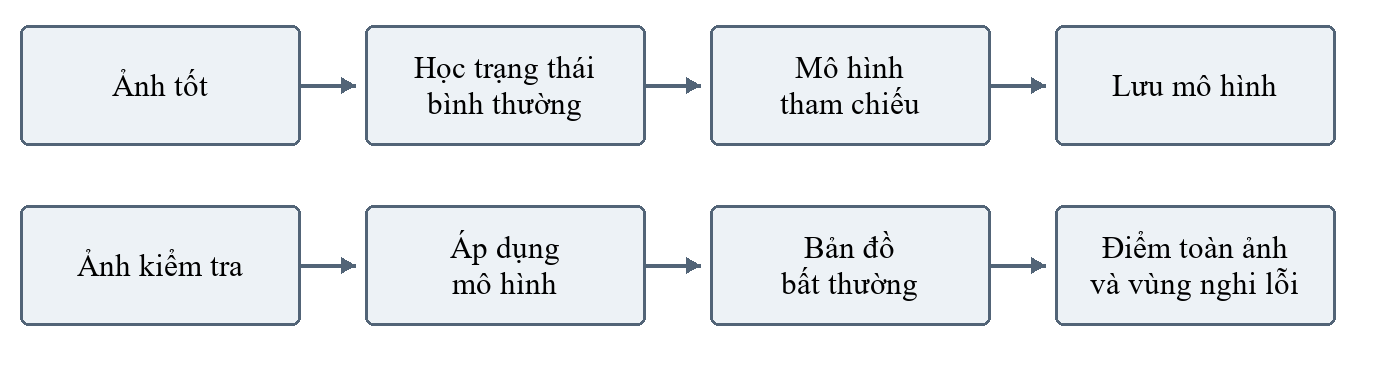
\includegraphics[width=0.9\linewidth]{images/img08.png}
  \caption{Quy trình tổng quát của bài toán phát hiện và định vị bất thường (Sơ đồ nguyên lý, không phải kết quả thực nghiệm)}
  \label{fig:overview}
\end{figure}

\section{Tổng quan các hướng tiếp cận}

\subsection{Phương pháp dựa trên tái tạo ảnh}

Các phương pháp tái tạo học một phép biến đổi để phục hồi đầu vào từ một biểu diễn trung gian. Khi chỉ được học trên ảnh tốt, mô hình được kỳ vọng tái tạo tốt các cấu trúc bình thường. Sự khác biệt giữa ảnh đầu vào và ảnh tái tạo là cơ sở xây dựng điểm bất thường. Autoencoder là mô hình tiêu biểu cho hướng tiếp cận này~\cite{goodfellowDeepLearning2016}.

Ưu điểm của hướng tái tạo là có thể quan sát trực tiếp ảnh đầu vào, ảnh phục hồi và bản đồ sai số. Tuy nhiên, giả thiết ảnh lỗi luôn có sai số tái tạo lớn không phải lúc nào cũng đúng. Mạng có thể tái tạo được cả vùng lỗi hoặc làm mờ các chi tiết bình thường, dẫn đến bỏ sót hoặc cảnh báo nhầm. Vì vậy, chất lượng tái tạo và khả năng phát hiện lỗi phải được đánh giá riêng.

\subsection{Phương pháp dựa trên đặc trưng học trước}

Một mạng nơ-ron tích chập đã được huấn luyện trước có thể được dùng làm bộ trích xuất đặc trưng. Thay vì chỉ so sánh màu sắc tại từng điểm ảnh, hệ thống làm việc với các vector mô tả kết cấu, đường nét và cấu trúc cục bộ. Đầu ra của các tầng trung gian vẫn giữ thông tin không gian, phù hợp với yêu cầu xác định vị trí bất thường.

Trong hướng này, trọng số của bộ trích xuất có thể được giữ cố định. Giai đoạn xây dựng mô hình trên ảnh tốt tập trung vào tính toán thống kê hoặc lưu giữ đặc trưng tham chiếu. Như vậy, việc sử dụng mạng học sâu không đồng nghĩa với việc phải huấn luyện lại toàn bộ mạng trên dữ liệu của đề tài. PaDiM và PatchCore là hai phương pháp nhóm dự kiến nghiên cứu theo hướng này~\cite{defardPaDiMPatchDistribution2021,rothTotalRecallIndustrial2022,nhom13MVTecAnomalyDetection2026}.

PaDiM mô hình hóa sự biến thiên của đặc trưng tại từng vị trí bằng các tham số thống kê. PatchCore lưu một tập đặc trưng bình thường đại diện rồi đối chiếu đặc trưng ảnh mới với tập đó. Hai cách biểu diễn này tạo ra những yêu cầu khác nhau về bộ nhớ, phép tính suy luận và mức độ phụ thuộc vào vị trí của vật thể.

\subsection{Phạm vi các phương pháp được lựa chọn}

Nhóm lựa chọn Autoencoder làm mô hình cơ sở để khảo sát hướng tái tạo; PaDiM và PatchCore là hai phương pháp chính để khảo sát hướng sử dụng đặc trưng học trước. Sự lựa chọn này cho phép đối chiếu ba cách biểu diễn trạng thái bình thường: trọng số của mạng tái tạo, phân phối thống kê và tập vector tham chiếu.

Việc so sánh không chỉ nhằm tìm phương pháp có AUROC cao hơn. Nhóm còn cần xem xét dạng lỗi bị bỏ sót, vùng cảnh báo nhầm và chi phí tài nguyên. Một phương pháp có chất lượng tốt trên bề mặt ít biến động chưa chắc giữ được ưu thế trên sản phẩm có tư thế thay đổi. Các nhận định về ưu thế thực tế chỉ được kết luận sau khi có kết quả trên dữ liệu của nhóm.

\section{Các mô hình và phương pháp sử dụng}

\subsection{Mô hình Autoencoder}

Autoencoder gồm bộ mã hóa và bộ giải mã. Bộ mã hóa chuyển ảnh đầu vào thành biểu diễn tiềm ẩn; bộ giải mã sử dụng biểu diễn đó để tái tạo ảnh. Với ảnh $x$, ký hiệu $f$ là bộ mã hóa, $g$ là bộ giải mã và $z$ là biểu diễn trung gian, quá trình truyền tiến có dạng~\cite{goodfellowDeepLearning2016}:
\begin{equation}
  z = f(x), \qquad \hat{x} = g(z) = g\bigl(f(x)\bigr)
  \label{eq:ae-forward}
\end{equation}

Đối với ảnh công nghiệp, một Autoencoder tích chập là hướng triển khai phù hợp để khai thác quan hệ lân cận giữa các điểm ảnh. Các lớp mã hóa giảm kích thước không gian và xây dựng đặc trưng; các lớp giải mã khôi phục kích thước đầu ra. Biểu diễn ở phần cổ chai giới hạn lượng thông tin truyền qua, buộc mô hình chọn lọc các cấu trúc cần thiết để phục hồi ảnh.

\begin{figure}[htbp]
  \centering
  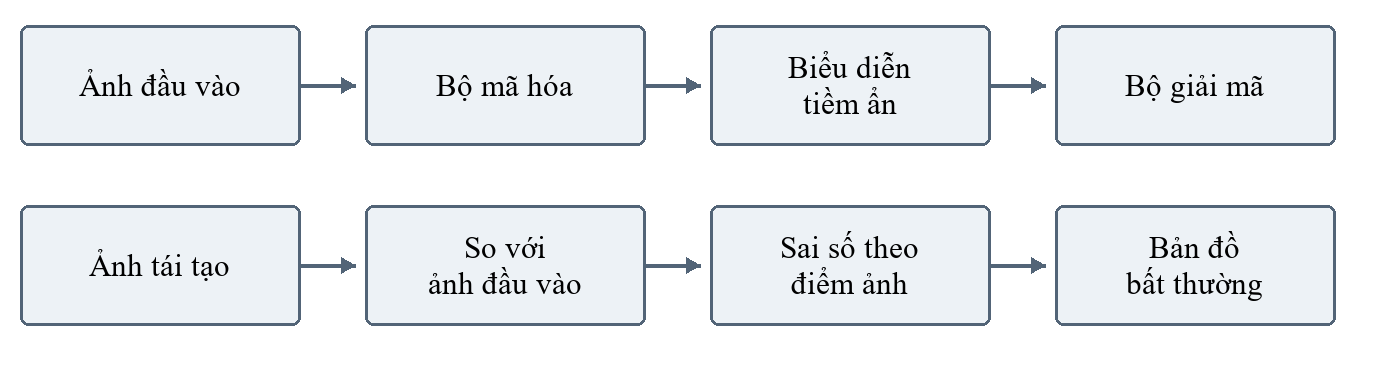
\includegraphics[width=0.9\linewidth]{images/img09.png}
  \caption{Nguyên lý tái tạo và tính bản đồ sai số của Autoencoder (Sơ đồ nguyên lý, không phải kết quả thực nghiệm)}
  \label{fig:ae}
\end{figure}

Một hàm mất mát khởi đầu có thể sử dụng là sai số bình phương trung bình. Với ảnh có chiều cao $H$, chiều rộng $W$ và $C$ kênh, mất mát tái tạo được viết như sau:
\begin{equation}
  L(x,\hat{x}) = \frac{1}{HWC}\sum_{u=1}^{H}\sum_{v=1}^{W}\sum_{c=1}^{C}
  \bigl[x(u,v,c) - \hat{x}(u,v,c)\bigr]^{2}
  \label{eq:ae-loss}
\end{equation}

Các tổng được lấy trên toàn bộ vị trí và kênh ảnh. Trong huấn luyện, giá trị mất mát được trung bình trên các mẫu trong lô dữ liệu; thuật toán tối ưu cập nhật trọng số để giảm sai số. Đầu vào và ảnh tái tạo phải có cùng kích thước và cùng thang giá trị thì phép so sánh mới có ý nghĩa.

Ở bước kiểm tra, sai số tại mỗi vị trí có thể được lấy trung bình theo các kênh màu để tạo bản đồ $A(u,v)$. Sau bước làm mượt nếu có, một cách tổng hợp đơn giản là lấy giá trị lớn nhất của bản đồ làm điểm bất thường của ảnh. Cách tổng hợp này nhạy với lỗi cục bộ, nhưng cũng có thể bị ảnh hưởng bởi một vài vị trí nhiễu có sai số cao.
\begin{equation}
  A(u,v) = \frac{1}{C}\sum_{c=1}^{C}\bigl[x(u,v,c) - \hat{x}(u,v,c)\bigr]^{2}
  \label{eq:ae-map}
\end{equation}

Kích thước cổ chai là một yếu tố cần khảo sát. Cổ chai quá nhỏ có thể làm mất các kết cấu bình thường; mạng có năng lực quá lớn lại có khả năng phục hồi cả chi tiết lỗi. Ngoài ra, sai số ở mức điểm ảnh dễ thay đổi theo điều kiện chiếu sáng và chất lượng ảnh. Đây là các giả thuyết cần đối chiếu bằng ảnh tái tạo và bản đồ bất thường, không phải kết quả đã được xác nhận trong đề tài.

Trong kế hoạch hiện tại, nhóm dự kiến tự xây dựng Autoencoder làm mốc so sánh. Số lớp, số kênh, kích thước biểu diễn tiềm ẩn, hàm mất mát, số epoch và tốc độ học chưa được xem là cấu hình cuối cùng. Các giá trị gợi ý trong kho mã nguồn chỉ là điểm xuất phát cho việc triển khai~\cite{nhom13MVTecAnomalyDetection2026}.

\subsection{Phương pháp PaDiM}

PaDiM, viết tắt của Patch Distribution Modeling, sử dụng đặc trưng từ CNN học trước để mô tả các vùng cục bộ của ảnh. Các đặc trưng ở nhiều tầng được đưa về lưới không gian tương ứng rồi ghép lại. Việc kết hợp các tầng cho phép biểu diễn chứa thông tin ở nhiều mức độ chi tiết~\cite{defardPaDiMPatchDistribution2021}.

Theo định hướng trong tài liệu dự án, bộ trích xuất được giữ cố định. Tại mỗi vị trí của lưới đặc trưng, nhóm thu các vector từ ảnh tốt, lựa chọn một tập chiều đặc trưng và ước lượng trung bình cùng ma trận hiệp phương sai. Các chỉ số chiều được chọn phải thống nhất giữa bước xây dựng mô hình và bước kiểm tra~\cite{nhom13MVTecAnomalyDetection2026}.

\begin{figure}[htbp]
  \centering
  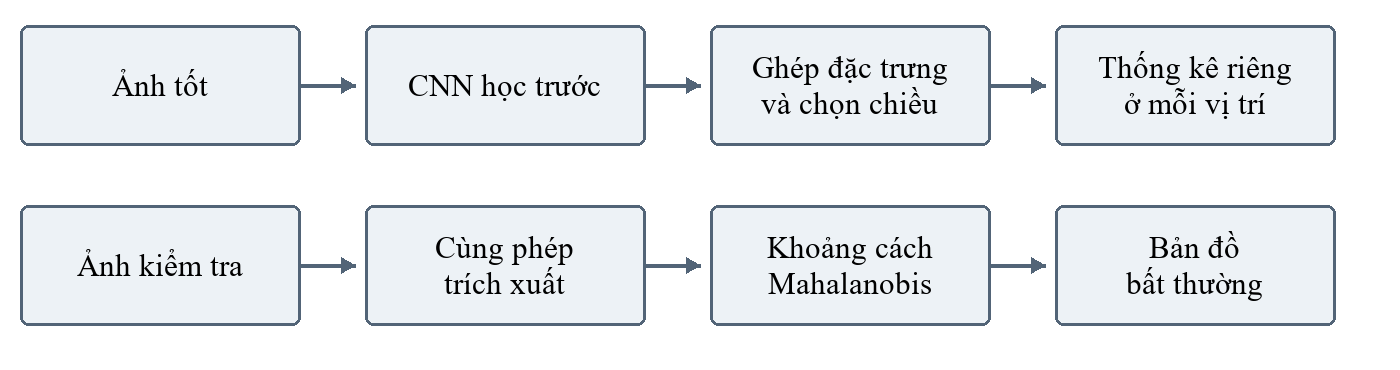
\includegraphics[width=0.9\linewidth]{images/img10.png}
  \caption{Luồng xử lý của PaDiM với thống kê riêng theo vị trí (Sơ đồ nguyên lý, không phải kết quả thực nghiệm)}
  \label{fig:padim}
\end{figure}

Gọi $z_k(p)$ là vector đặc trưng của ảnh huấn luyện thứ $k$ tại vị trí $p$; $N$ là số ảnh tốt. Các công thức thống kê mẫu được sử dụng để mô tả tập vector tại vị trí đó:
\begin{align}
  \mu_p &= \frac{1}{N}\sum_{k=1}^{N} z_k(p) \label{eq:padim-mean}\\
  \Sigma_p &= \frac{1}{N-1}\sum_{k=1}^{N}\bigl[z_k(p)-\mu_p\bigr]\bigl[z_k(p)-\mu_p\bigr]^{\top} + \varepsilon I \label{eq:padim-cov}
\end{align}

Trong đó $I$ là ma trận đơn vị và $\varepsilon$ là một số dương nhỏ. Thành phần $\varepsilon I$ hỗ trợ ổn định phép tính khi ma trận hiệp phương sai gần suy biến, đặc biệt khi số chiều đặc trưng lớn so với số mẫu. Giá trị $\varepsilon$ là một tham số triển khai cần được ghi lại để tái lập kết quả.

Với vector $z(p)$ của ảnh kiểm tra, khoảng cách Mahalanobis tới thống kê bình thường được dùng làm điểm bất thường tại vị trí $p$:
\begin{equation}
  d_p = \sqrt{\bigl[z(p)-\mu_p\bigr]^{\top}\,\Sigma_p^{-1}\,\bigl[z(p)-\mu_p\bigr]}
  \label{eq:padim-mahalanobis}
\end{equation}

Khác với khoảng cách Euclid thuần túy, biểu thức này có xét đến độ biến thiên và tương quan giữa các chiều. Một sai lệch trên chiều đặc trưng vốn ổn định có thể đáng chú ý hơn một sai lệch cùng độ lớn trên chiều thường xuyên biến động. Các điểm $d_p$ được sắp về lưới không gian và nội suy để tạo bản đồ bất thường ở kích thước đánh giá.

Điểm cần lưu ý trong kế hoạch triển khai là PaDiM lưu thống kê riêng cho từng vị trí. Khi vật thể dịch chuyển hoặc xoay, cùng một vị trí có thể nhận các cấu trúc khác nhau giữa những ảnh tốt. Nhóm cần kiểm tra ảnh hưởng này trên các loại sản phẩm thích hợp. Bộ nhớ lưu ma trận cũng tăng nhanh khi tăng số chiều; vì vậy lựa chọn số chiều phải cân nhắc cùng độ phân giải của lưới đặc trưng~\cite{nhom13MVTecAnomalyDetection2026}.

ResNet18, các tầng trích xuất và số chiều đặc trưng trong tài liệu dự án hiện mới mang tính gợi ý. Báo cáo sẽ ghi đúng backbone, tầng, phép giảm chiều và tham số ổn định hóa sau khi nhóm lựa chọn và chạy thực nghiệm.

\subsection{Phương pháp PatchCore}

PatchCore biểu diễn trạng thái bình thường bằng một bộ nhớ chứa các vector đặc trưng cục bộ đại diện. Phương pháp sử dụng CNN học trước, tổng hợp đặc trưng vùng lân cận và chọn một tập con đại diện để giảm lượng dữ liệu cần lưu. Khi kiểm tra, đặc trưng mới được so với các vector gần nhất trong bộ nhớ~\cite{rothTotalRecallIndustrial2022}.

Theo phương án nghiên cứu của nhóm, giai đoạn xây dựng bộ nhớ bắt đầu từ ảnh tốt của từng loại sản phẩm. Sau khi trích xuất đặc trưng, các vector cục bộ được tập hợp vào một tập chung. Khác với việc lập một phân phối riêng cho từng tọa độ, phép tra cứu sử dụng các mẫu tham chiếu trong bộ nhớ mà không buộc vector phải đến từ đúng vị trí ảnh ban đầu~\cite{nhom13MVTecAnomalyDetection2026}.

\begin{figure}[htbp]
  \centering
  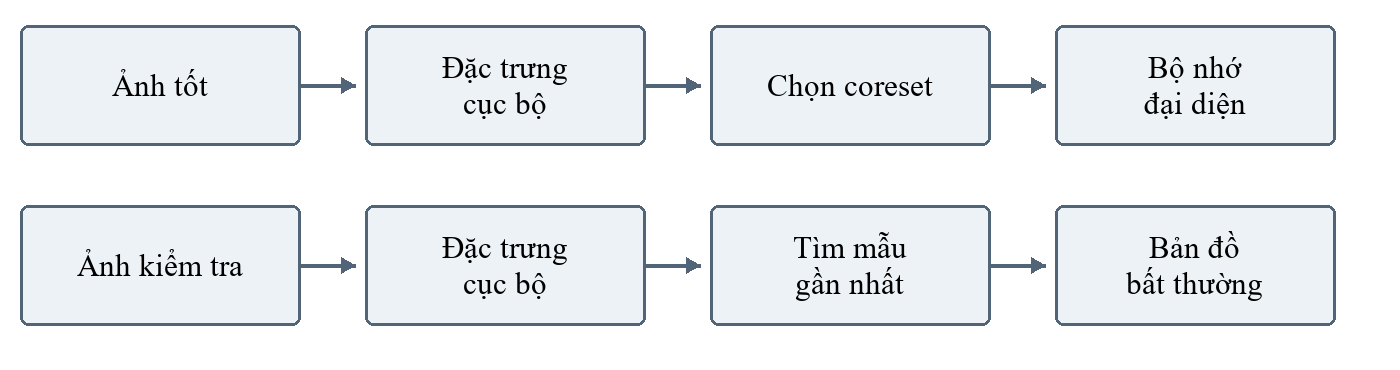
\includegraphics[width=0.9\linewidth]{images/img11.png}
  \caption{Nguyên lý xây dựng bộ nhớ và tra cứu của PatchCore (Sơ đồ nguyên lý, không phải kết quả thực nghiệm)}
  \label{fig:patchcore}
\end{figure}

Lưu toàn bộ vector có thể tạo ra nhiều mẫu gần giống nhau. Bước chọn tập con đại diện, gọi là coreset, nhằm giảm sự dư thừa trong khi vẫn giữ độ bao phủ của không gian đặc trưng. Tỷ lệ giữ lại là một yếu tố cần khảo sát: tập quá nhỏ có thể bỏ mất biến thiên bình thường, còn tập lớn tăng chi phí lưu trữ và tìm kiếm.

Gọi $M$ là tập vector đã được chọn và $q$ là vector của một vùng trong ảnh kiểm tra. Điểm bất thường cục bộ cơ bản có thể được diễn giải bằng khoảng cách tới mẫu gần nhất:
\begin{equation}
  a(q) = \min_{m \in M}\,\lVert q - m\rVert_{2}
  \label{eq:patchcore-score}
\end{equation}

Nếu $q$ ở xa các vector bình thường được lưu, vùng đó nhận điểm cao. Sau khi tính cho các vị trí, các điểm được đưa về lưới ảnh để tạo bản đồ bất thường. Công thức trên mô tả điểm cục bộ; cách tạo điểm cho toàn ảnh còn tùy phiên bản triển khai. Bài báo PatchCore có bước điều chỉnh trọng số khi tính điểm ảnh, nên không nên mặc nhiên coi mọi bản dùng giá trị cực đại đơn giản là tái hiện đầy đủ phương pháp gốc~\cite{rothTotalRecallIndustrial2022}.

Trong đề tài, nhóm cần ghi rõ cách tính điểm ảnh khi sử dụng thư viện hoặc tự cài đặt. Giao thức chung cho phép mỗi phương pháp tạo điểm ảnh của mình; khi không có cách riêng, hàm đánh giá chung sử dụng giá trị lớn nhất của bản đồ đã làm mượt. Mọi thay đổi về cách tổng hợp phải được lưu cùng cấu hình chạy~\cite{nhom13MVTecAnomalyDetection2026}.

Việc bỏ ràng buộc khớp đúng vị trí tạo cơ hội nhận diện các vùng bình thường khi vật thể thay đổi tư thế, nhưng không bảo đảm bất biến với mọi phép xoay hoặc dịch chuyển. Kết quả vẫn phụ thuộc vào đặc trưng học trước và mức độ bao phủ của bộ nhớ. Những lỗi về quan hệ giữa các bộ phận cũng cần được phân tích, vì từng vùng nhỏ có thể vẫn giống mẫu bình thường dù bố cục tổng thể đã sai.

Trong kế hoạch phân công, hai thành viên cùng thực hiện PatchCore trên các nhóm loại sản phẩm khác nhau. Vì vậy, backbone, tầng trích xuất, tỷ lệ coreset, seed và cách tính điểm phải thống nhất trước khi tổng hợp kết quả. Cấu hình gợi ý hiện có trong kho mã nguồn chưa phải cấu hình thực nghiệm đã chốt~\cite{nhom13MVTecAnomalyDetection2026}.

\section{Lý do lựa chọn các phương pháp cho đề tài}

Ba phương pháp được lựa chọn cùng đáp ứng điều kiện xây dựng mô hình từ ảnh tốt và có khả năng tạo bản đồ bất thường. Autoencoder giúp nhóm thực hành thiết kế mạng, lan truyền ngược và tối ưu tham số. PaDiM bổ sung cách tiếp cận thống kê trên đặc trưng học sâu, còn PatchCore cho phép khảo sát cách lưu giữ và tìm kiếm các mẫu đặc trưng đại diện.

Về nội dung học phần, bộ phương pháp này liên kết kiến thức mạng nơ-ron, biểu diễn đặc trưng, đại số tuyến tính và đánh giá mô hình với một bài toán thống nhất. Về thực nghiệm, chúng tạo điều kiện phân tích sự đánh đổi giữa chất lượng phát hiện, bộ nhớ và thời gian suy luận. Bảng~\ref{tab:compare} tổng hợp khác biệt về nguyên lý; bảng không biểu thị thứ hạng hiệu năng của các mô hình do nhóm triển khai.

\begin{table}[htbp]
  \centering
  \caption{So sánh nguyên lý của ba phương pháp}
  \label{tab:compare}
  \small
  \begin{tabular}{@{}>{\raggedright\arraybackslash}p{3cm} >{\raggedright\arraybackslash}p{3.2cm} >{\raggedright\arraybackslash}p{3.7cm} >{\raggedright\arraybackslash}p{3.7cm}@{}}
    \toprule
    Tiêu chí & Autoencoder & PaDiM & PatchCore \\
    \midrule
    Biểu diễn bình thường & Trọng số mạng tái tạo & Trung bình, hiệp phương sai theo vị trí & Tập vector đặc trưng đại diện \\
    Bước xây dựng & Tối ưu trọng số mạng & Trích xuất và tính thống kê & Trích xuất và chọn coreset \\
    Điểm cục bộ & Sai số tái tạo & Khoảng cách Mahalanobis & Khoảng cách tới mẫu gần nhất \\
    Điểm cần khảo sát & Tái tạo mờ hoặc tái tạo cả lỗi & Phụ thuộc vị trí và số chiều & Kích thước bộ nhớ và chi phí tìm kiếm \\
    \bottomrule
  \end{tabular}
\end{table}

Không có căn cứ để khẳng định trước một phương pháp luôn tốt hơn hai phương pháp còn lại trên mọi loại sản phẩm. Nhóm dự kiến xem xét cả kết quả trung bình và kết quả riêng từng loại, đồng thời đối chiếu ảnh gốc, mặt nạ chuẩn và bản đồ dự đoán. Cách phân tích này giúp phân biệt lỗi bỏ sót, cảnh báo nhầm trên nền và trường hợp xác định đúng ảnh có lỗi nhưng khoanh vùng chưa chính xác.

\section{Định hướng triển khai và đánh giá}

Theo giao thức trong kho mã nguồn, mỗi phương pháp được xây dựng riêng cho từng loại của MVTec AD, chỉ sử dụng thư mục \texttt{train/good} trong giai đoạn học trạng thái bình thường. Tập test được giữ cho đánh giá cuối cùng; nhóm không điều chỉnh siêu tham số dựa trên kết quả của tập này. Nếu cần xác thực trong quá trình phát triển, cách tách dữ liệu phải được mô tả và bảo đảm độc lập với tập kiểm thử~\cite{nhom13MVTecAnomalyDetection2026}.

Bản đồ bất thường đưa vào bộ đánh giá có kích thước $256 \times 256$ và phải khớp tọa độ với mặt nạ chuẩn. Khi đổi kích thước mặt nạ nhị phân, nhóm sử dụng nội suy lân cận gần nhất để giữ nhãn 0/1. Độ phân giải bên trong mô hình có thể khác, nhưng bước chuyển đổi về kích thước đánh giá phải được thực hiện nhất quán. Thứ tự ảnh, nhãn, mặt nạ và bản đồ dự đoán cũng phải trùng nhau.

Image-AUROC được tính từ điểm toàn ảnh và nhãn tốt hoặc lỗi; pixel-AUROC được tính từ điểm tại các pixel và mặt nạ vùng lỗi. AUROC đánh giá khả năng xếp hạng khi thay đổi ngưỡng, không yêu cầu chọn trước một ngưỡng phân loại duy nhất~\cite{scikit-learnRocAucScore}. Các chỉ số được tính riêng từng loại rồi lấy trung bình theo loại; không gộp điểm của các loại có thang đo khác nhau để thay cho phép tính này.

Để trình diễn ảnh tốt hoặc lỗi bằng nhãn nhị phân, hệ thống vẫn cần một ngưỡng quyết định. Ngưỡng hiển thị này phải được xác định theo quy trình riêng và ghi rõ căn cứ lựa chọn; không được dùng nhãn của tập test để điều chỉnh rồi báo cáo như đánh giá độc lập. Tương tự, chuẩn hóa màu cho từng ảnh có thể giúp quan sát bản đồ, nhưng không nên làm thay đổi các điểm số dùng tính AUROC.

Ngoài chất lượng phát hiện, nhóm dự kiến ghi thời gian xây dựng mô hình, thời gian suy luận trên mỗi ảnh và dung lượng lưu mô hình. Thiết bị, cách đo, số mẫu và việc tính hay loại trừ thời gian đọc dữ liệu phải được mô tả để việc so sánh có ý nghĩa. Với PaDiM, thời gian xây dựng gồm trích xuất đặc trưng và tính thống kê; với PatchCore, thời gian này gồm cả quá trình tạo và rút gọn bộ nhớ.

Các thông tin cần bổ sung sau triển khai gồm kiến trúc Autoencoder, backbone và tầng đặc trưng, số chiều của PaDiM, tỷ lệ coreset của PatchCore, quy tắc làm mượt, cách tính điểm ảnh và cấu hình phần cứng. Kết quả thực nghiệm, hình dự đoán thực tế và nhận xét dựa trên số liệu sẽ được trình bày ở chương tiếp theo. Nội dung hiện tại là cơ sở phương pháp và kế hoạch đánh giá, chưa phải báo cáo hoàn thành huấn luyện.

\chapter{THỰC NGHIỆM VÀ ĐÁNH GIÁ}

\section{Nguồn kết quả và cấu hình thực nghiệm}

Kết quả trong chương này lấy từ 45 dòng của tệp \path{results/results.csv}: ba phương pháp, mỗi phương pháp đủ 15 loại MVTec AD. Đây là kết quả thực nghiệm của nhóm ngày 25/10/2026 trên Google Colab với GPU Tesla T4, được giữ nguyên khi bổ sung demo. Các bảng được sinh trực tiếp bằng \path{tools/report_results.py}; mã băm và số dòng nằm trong \path{docs/results_provenance.json}. Không thay số liệu Colab bằng số chạy bổ sung trên máy cá nhân.

Tất cả phương pháp chỉ học từ \texttt{train/good}, resize ảnh và mặt nạ về $256\times256$; mặt nạ dùng nội suy lân cận gần nhất. Nhãn tốt/lỗi và mặt nạ test chỉ phục vụ tính AUROC. Điểm được đo riêng từng loại rồi lấy trung bình đều giữa các loại; số tổng hợp không phải AUROC gộp mọi ảnh hoặc mọi pixel của 15 loại.

Autoencoder là mạng tích chập tự xây, latent 256, huấn luyện 100 epoch với MSE, Adam, learning rate $10^{-3}$, batch 16 và làm mượt bản đồ với $\sigma=4$. Đầu vào AE nằm trong $[0,1]$. PaDiM dùng ResNet-18 học trước trên ImageNet, lấy đặc trưng layer1--3 và số chiều mặc định của Anomalib 2.7.0. PatchCore dùng Wide-ResNet-50-2, layer2--3, coreset 10\% và 9 láng giềng. Hai phương pháp đặc trưng dùng chuẩn hóa ImageNet. Cấu hình resize, seed 42 và bộ đánh giá được dùng chung; phép chuẩn hóa theo yêu cầu từng mô hình được ghi riêng.

\section{Kết quả định lượng}

\begin{table}[htbp]\centering
\caption{Image-AUROC theo từng loại (kết quả Colab gốc).}
\begin{tabular}{@{}lrrr@{}}\toprule Loại & AE & PaDiM & PatchCore \\ \midrule
carpet & 0.553 & \textbf{0.988} & 0.988 \\
grid & 0.857 & 0.829 & \textbf{0.990} \\
leather & 0.807 & 0.999 & \textbf{1.000} \\
tile & 0.765 & 0.943 & \textbf{1.000} \\
wood & 0.938 & 0.966 & \textbf{0.987} \\
bottle & 0.926 & 0.998 & \textbf{1.000} \\
cable & 0.579 & 0.838 & \textbf{0.988} \\
capsule & 0.689 & 0.903 & \textbf{0.994} \\
hazelnut & 0.923 & 0.720 & \textbf{1.000} \\
metal\_nut & 0.574 & 0.957 & \textbf{0.997} \\
pill & 0.603 & 0.824 & \textbf{0.942} \\
screw & 0.579 & 0.752 & \textbf{0.964} \\
toothbrush & \textbf{0.958} & 0.772 & 0.917 \\
transistor & 0.807 & 0.943 & \textbf{0.995} \\
zipper & 0.775 & 0.927 & \textbf{0.977} \\
\midrule Texture & 0.784 & 0.945 & 0.993 \\
Object & 0.741 & 0.863 & 0.977 \\
Tất cả & 0.756 & 0.890 & 0.983 \\
\bottomrule\end{tabular}\end{table}
\begin{table}[htbp]\centering
\caption{Pixel-AUROC theo từng loại (kết quả Colab gốc).}
\begin{tabular}{@{}lrrr@{}}\toprule Loại & AE & PaDiM & PatchCore \\ \midrule
carpet & 0.805 & 0.989 & \textbf{0.991} \\
grid & 0.844 & 0.916 & \textbf{0.981} \\
leather & 0.916 & 0.987 & \textbf{0.992} \\
tile & 0.559 & 0.905 & \textbf{0.955} \\
wood & 0.780 & 0.922 & \textbf{0.930} \\
bottle & 0.935 & 0.978 & \textbf{0.986} \\
cable & 0.876 & 0.953 & \textbf{0.985} \\
capsule & 0.531 & 0.983 & \textbf{0.990} \\
hazelnut & 0.968 & 0.972 & \textbf{0.988} \\
metal\_nut & 0.887 & 0.941 & \textbf{0.987} \\
pill & 0.887 & 0.944 & \textbf{0.981} \\
screw & 0.965 & 0.974 & \textbf{0.989} \\
toothbrush & 0.932 & 0.985 & \textbf{0.989} \\
transistor & 0.899 & \textbf{0.976} & 0.973 \\
zipper & 0.865 & 0.970 & \textbf{0.981} \\
\midrule Texture & 0.781 & 0.944 & 0.970 \\
Object & 0.874 & 0.967 & 0.985 \\
Tất cả & 0.843 & 0.960 & 0.980 \\
\bottomrule\end{tabular}\end{table}

\clearpage

Trên trung bình 15 loại, PatchCore đạt image-AUROC xấp xỉ 0,983 và pixel-AUROC 0,980; PaDiM lần lượt đạt 0,890 và 0,960; Autoencoder đạt 0,756 và 0,843. Trong cấu hình đã chạy, mô hình đặc trưng học trước có kết quả trung bình cao hơn mạng tái tạo học từ đầu. Đây là kết luận cho lần chạy và backbone nêu trên, không chứng minh thứ hạng phổ quát của các thuật toán.

PatchCore có kết quả phát hiện tốt ở nhiều loại như bottle, hazelnut, leather và tile, nhưng giảm ở toothbrush và pill. Autoencoder đạt image-AUROC cao nhất trong ba phương pháp ở toothbrush (khoảng 0,958), cho thấy trung bình cao hơn không đồng nghĩa thắng ở mọi loại. AE yếu ở carpet, cable, metal\_nut và screw; pixel-AUROC của tile và capsule gần mức ngẫu nhiên. Có thể kiểm tra giả thuyết tái tạo mờ hoặc tái tạo cả lỗi bằng ảnh dự đoán; chỉ số đơn lẻ chưa đủ để khẳng định nguyên nhân.

PaDiM dùng ràng buộc thống kê theo vị trí; ảnh vật thể thay đổi tư thế có thể gây sai lệch. Kết quả image-AUROC thấp ở hazelnut, screw và toothbrush cho thấy cần xem xét sai số theo loại thay vì chỉ nêu trung bình. Không điều chỉnh cấu hình dựa trên các loại test yếu rồi coi số mới là đánh giá độc lập.

\section{Chi phí và giới hạn phép đo}

Trong CSV Colab, tổng thời gian xây dựng 15 mô hình khoảng 22 phút cho AE, 6 phút cho PaDiM và 30 phút cho PatchCore. Đây là số của một lần chạy, chưa có lặp seed để ước lượng phương sai. Thời gian suy luận AE trung bình khoảng 44,8 ms/ảnh bao gồm đọc dữ liệu từ Drive, còn PaDiM khoảng 5,5 ms và PatchCore khoảng 35,5 ms chỉ đo lượt chạy mô hình. Vì phạm vi đo khác nhau, không dùng ba số này để kết luận AE chậm hơn hoặc nhanh hơn hai mô hình còn lại.

Dung lượng trong CSV cũng cần phân biệt: AE là trọng số mạng, PaDiM chủ yếu là thống kê Gauss, PatchCore chủ yếu là memory bank. Backbone học trước có thể chưa được tính cùng phạm vi nên đây chưa phải phép so sánh tổng bộ nhớ triển khai. Checkpoint tự mô tả bổ sung cho demo lưu cả state dict của mô hình; kích thước tệp thực tế không nhất thiết bằng cột memory trong CSV gốc.

\section{Demo và khả năng chạy lại}

Demo Gradio nhận ảnh, loại sản phẩm và một trong ba phương pháp; trả về điểm bất thường, heatmap chồng ảnh và nhận xét theo ngưỡng từng loại. Điểm là độ bất thường, không phải xác suất sản phẩm lỗi. Heatmap dùng thang cố định được suy ra từ ảnh train tốt, tránh việc chuẩn hóa từng ảnh khiến cả ảnh tốt cũng hiện vùng đỏ mạnh.

Trọng số AE đã được lưu từ lần huấn luyện trước. PaDiM và PatchCore được fit bổ sung để lưu đầy đủ tham số Gauss và memory bank. Lần bổ sung chạy trên RTX 3050 Laptop GPU, batch 4, chỉ dùng train/good để fit; CSV bổ sung nằm riêng ở \path{results/demo_models/results.csv}. Không coi checkpoint bổ sung là chính các trọng số Colab đã mất và không gộp thời gian giữa hai thiết bị.

Ngưỡng demo là phân vị 99,5\% của điểm trên tối đa 64 ảnh train tốt đã tham gia fit. Vì đây là mẫu trong huấn luyện, ngưỡng chỉ mang tính tham khảo và không bảo đảm tỷ lệ báo động giả 0,5\% trên ảnh mới. Nhãn test không được dùng để chọn ngưỡng. Một bước phát triển tiếp theo là tách tập ảnh tốt độc lập để hiệu chỉnh và đo độ ổn định ngưỡng. AUROC trong hai bảng không phụ thuộc quyết định ngưỡng này.

Checkpoint đi kèm cấu hình chuẩn hóa, kích thước ảnh và phương pháp; demo nạp trọng số thay vì huấn luyện lại mỗi lần người dùng gửi ảnh. Có thể tiếp tục tạo từng mô hình sau gián đoạn. Dữ liệu và checkpoint nằm ngoài Git theo quy định kho mã nguồn; mã nguồn, CSV, cấu hình và hướng dẫn chạy được lưu trên nhánh riêng để rà soát.

\section{Kết luận và phần cần mở rộng}

Trong phạm vi một lần chạy trên MVTec AD, PatchCore cho trung bình AUROC cao nhất; PaDiM có thời gian xây dựng thấp hơn trong cùng môi trường Colab; AE cung cấp baseline tái tạo tự xây và vẫn có loại đạt kết quả tốt. Các hạn chế còn lại gồm độ biến thiên giữa seed, phép đo tài nguyên chưa đồng nhất và ngưỡng demo chưa được kiểm chứng ngoài mẫu. Cần bổ sung giao thức đo model-only thống nhất, tập calibration độc lập và phân tích hình ảnh của các ca bỏ sót trước khi đưa ra kết luận triển khai thực tế.

\chapter*{KẾT LUẬN}
\addcontentsline{toc}{chapter}{KẾT LUẬN}

Đề tài đã xây dựng và đánh giá ba phương pháp phát hiện và định vị bất thường không giám sát trên đủ 15 loại của
MVTec AD theo cùng một giao thức. Autoencoder do nhóm tự thiết kế và huấn luyện; PaDiM và PatchCore dùng đặc trưng
học trước qua thư viện Anomalib.

Kết quả cho thấy PatchCore tốt nhất (image-AUROC 0,983, pixel-AUROC 0,980), sát số liệu của bài báo gốc. PaDiM đứng
thứ hai (0,890 và 0,960), nhanh nhất, nhưng điểm ảnh kém tin cậy ở các loại vật thể xoay. Autoencoder thấp nhất
(0,756 và 0,843): bản tái tạo mờ làm sai số xuất hiện ở viền và nền thay vì ở vùng lỗi, dù phương pháp vẫn tốt ở các
loại có lỗi lớn như toothbrush. Trong phạm vi thực nghiệm này, dùng lại đặc trưng ImageNet hiệu quả hơn nhiều so
với học tái tạo ảnh từ đầu trên vài trăm ảnh tốt.

Các hướng phát triển xuất phát trực tiếp từ hạn chế ở Chương 3:
\begin{itemize}
  \item Chạy Autoencoder với nhiều seed và thử hàm mất mát SSIM~\cite{bergmannImprovingUnsupervisedDefect2019} để
        biết phần nào của khoảng cách là do cấu hình.
  \item Chạy PaDiM và PatchCore với cùng backbone để tách ảnh hưởng của cơ chế khỏi ảnh hưởng của backbone.
  \item Chọn ngưỡng quyết định từ một tập ảnh tốt tách riêng và đo tỷ lệ báo động giả, làm cơ sở cho việc dùng mô
        hình trong một hệ thống kiểm tra thực tế.
\end{itemize}


\printbibliography[heading=bibintoc,title={TÀI LIỆU THAM KHẢO}]

\chapter*{PHỤ LỤC. MÃ NGUỒN VÀ CÁCH TÁI LẬP}
\addcontentsline{toc}{chapter}{PHỤ LỤC. MÃ NGUỒN VÀ CÁCH TÁI LẬP}

\section*{Kho mã nguồn}

Toàn bộ mã nguồn, cấu hình và tệp kết quả nằm trong kho mã nguồn của nhóm~\cite{nhom13MVTecAnomalyDetection2026}:
\begin{center}
  \url{https://github.com/AnDpTri/mvtec-anomaly-detection}
\end{center}
Kết quả trong Chương 3 được tạo từ commit \texttt{a839dd0} (PaDiM,
PatchCore) và \texttt{37fb3e5} (Autoencoder).

\begin{table}[htbp]
  \centering
  \small
  \begin{tabular}{@{}>{\raggedright\arraybackslash}p{6.1cm} >{\raggedright\arraybackslash}p{8.3cm}@{}}
    \toprule
    Thư mục & Nội dung \\
    \midrule
    \texttt{configs/common.yaml} & Cấu hình chung: kích thước ảnh, chuẩn hóa, seed, danh sách 15 loại \\
    \texttt{src/data/} & Đọc ảnh, mặt nạ và nhãn của MVTec AD \\
    \texttt{src/evaluation/} & Tính AUROC, vẽ hình minh họa, ghi và tổng hợp kết quả \\
    \texttt{src/autoencoder/} & Kiến trúc, huấn luyện và đánh giá Autoencoder \\
    \texttt{src/padim/}, \texttt{src/patchcore/} & Chạy PaDiM và PatchCore \\
    \texttt{src/common/} & Tiện ích chung, gồm lớp gọi mô hình của Anomalib \\
    \texttt{notebooks/colab\_run\_all.ipynb} & Notebook chạy toàn bộ thực nghiệm trên Google Colab \\
    \bottomrule
  \end{tabular}
\end{table}

\section*{Dữ liệu}

Đường tải chính thức của MVTec AD không còn truy cập được khi thực hiện đề tài; nhóm dùng bản sao trên Hugging Face
(\texttt{foersben/mvtec-ad}), cùng cấu trúc thư mục và số ảnh như Bảng~\ref{tab:mvtec}. Lệnh
\texttt{python tools/download\_mvtec.py <thư mục>} tải về đủ 15 loại.

\section*{Chạy lại thực nghiệm}

Từ thư mục gốc của kho mã nguồn, sau khi cài các thư viện trong \texttt{requirements.txt}:
\begin{verbatim}
python -m src.autoencoder.train --data-root <thư mục MVTecAD>
python -m src.padim.run         --data-root <thư mục MVTecAD>
python -m src.patchcore.run     --data-root <thư mục MVTecAD>
python -m src.evaluation.summary
\end{verbatim}
Mỗi lệnh chạy đủ 15 loại, ghi một dòng vào \texttt{results/results.csv} sau mỗi loại và bỏ qua các loại đã có kết
quả, nên có thể chạy tiếp sau khi bị gián đoạn. Lệnh cuối in bảng AUROC theo loại và trung bình theo nhóm như
Bảng~\ref{tab:summary} và Bảng~\ref{tab:per-category}.


\end{document}
